% --- ETUDE DE CAS ---
\section*{Étude de cas: Chiffrement}
\addcontentsline{toc}{section}{Étude de cas: Chiffrement}

\section*{AAV}
\addcontentsline{toc}{section}{AAV}
\begin{itemize}
  \item [4] Comparer différentes technologies de tunnelisation
  \item [4] Construire une PKI
  \item [2] Expliquer le fonctionnement des certificats numériques
  \item [2] Expliquer les termes de base liés à la cryptographie
  \item [3] Appliquer un système de codage simple
  \item [4] Sélectionner différentes solutions pour assurer la confidentialité d'un système X
\end{itemize}

\subsection*{Mots clés}
\phantomsection
\addcontentsline{toc}{subsection}{Mots clés}
\begin{itemize}
  \item Bcrypt
  \item Certificat Auto-signé
  \item VPN
  \item PKI
  \item Hachage
  \item Wildcard
  \item Client OpenVPN
  \item Tunnel VPN
  \item SSL
  \item TLS
  \item SSH
  \item GLPI
  \item POC
  \item LDAPS (LDAP via SSL/TLS)
  \item Cryptologie
  \item Chiffrement/Déchiffrement 
\end{itemize}

\subsection*{Contexte}
\phantomsection
\addcontentsline{toc}{subsection}{Contexte}
BERRIA prévoit de mettre en production une interface Web GLPI pour la gestion des tickets. Leila, la stagiaire, est chargée de définir la méthode d'authentification des utilisateurs et de sécuriser l'accès (utilisé en local et en télétravail). L'architecture réseau (DMZ ou VPN) et la gestion des certificats sont encore en discussion.

\subsection*{Problématique}
\phantomsection
\addcontentsline{toc}{subsection}{Problématique}
Comment sécuriser l'accès et l'authentification des utilisateurs locaux et distants à l'interface GLPI ?

\newpage

\subsection*{Contraintes}
\phantomsection
\addcontentsline{toc}{subsection}{Contraintes}
\begin{itemize}
  \item Budget
  \item Mobilité
  \item Authentification
  \item Sécurité
\end{itemize}

\subsection*{Généralisation}
\phantomsection
\addcontentsline{toc}{subsection}{Généralisation}
\begin{itemize}
  \item Cryptographie (Symétrique / Asymétrique)
  \item Authentification
  \item Sécurité des réseaux
  \item Infrastructure à Clés Publiques (PKI)
  \item Protocoles de communication sécurisés
  \item Tunnelisation

\end{itemize}

\subsection*{Livrables}
\phantomsection
\addcontentsline{toc}{subsection}{Livrables}
\begin{itemize}
  \item Architecture de la solution : Schéma réseau montrant le positionnement du serveur (DMZ vs LAN) et les flux.
  \item Proposition technique : Choix argumentés pour le certificat (PKI interne vs Public) et le mode d'accès (VPN vs HTTPS direct).
  \item Documentation de configuration : Procédure pour la mise en place du certificat et de l'authentification LDAPS.
  \item Maquette fonctionnelle : Preuve de concept (POC) validant l'accès sécurisé sans avertissement navigateur
\end{itemize}

\subsection*{Pistes de solutions}
\phantomsection
\addcontentsline{toc}{subsection}{Pistes de solutions}
\begin{itemize}
  \item Se renseigner sur le fonctionnement et le déploiement d'une PKI interne (Microsoft AD CS ou OpenSSL).
  \item Comparer les avantages et inconvénients d'un accès via VPN (OpenVPN) par rapport à une exposition directe en HTTPS (Reverse Proxy).
  \item Étudier le fonctionnement de l'authentification LDAPS et la configuration nécessaire côté serveur et client.
  \item Analyser les différences entre les certificats auto-signés, les certificats émis par une CA interne et les certificats publics (Wildcard).
  \item Distinguer clairement les notions de SSH, SSL et TLS.
\end{itemize}

\subsection*{Pistes de solutions}
\phantomsection
\addcontentsline{toc}{subsection}{Pistes de solutions}
\begin{itemize}
  \item Définir les mots clés (Cryptographie, PKI, VPN, TLS, etc.).
  \item Analyser les besoins de sécurité (Confidentialité, Intégrité, Authenticité) pour GLPI.
  \item Étudier le fonctionnement théorique du chiffrement et des certificats numériques.
  \item Comparer les solutions d'accès distant (VPN vs Publication Web sécurisée).
  \item Maquetter l'authentification LDAPS avec l'Active Directory.
  \item Mettre en place la solution de certificat choisie (résolution de l'avertissement navigateur).
  \item Configurer l'accès distant selon l'architecture retenue.
  \item Tester et valider la solution finale.
\end{itemize}

\clearpage
\section*{Démarche: Chiffrement}
\addcontentsline{toc}{section}{Démarche: Chiffrement}

\subsection*{Définition: Mots clés}
\phantomsection
\addcontentsline{toc}{subsection}{Définition: Mots clés}

\medskip
\noindent \textbf{Bcrypt}:\\
Bcrypt est une fonction de hachage adaptative conçue pour le stockage sécurisé des mots de passe. Elle rend les attaques par force brute très coûteuses grâce à un mécanisme volontairement lent et ajustable via un paramètre appelé \textit{cost}. Plus ce cost est élevé, plus le temps nécessaire pour générer un hash augmente, ce qui ralentit drastiquement les attaques, même avec du matériel spécialisé comme les GPU ou les ASIC. 

\noindent Dans la pratique, Bcrypt intègre un \textit{salt} unique et encode dans le hash final toutes les informations nécessaires (version, cost, salt, empreinte). En entreprise, il est utilisé pour sécuriser les bases utilisateurs des applications internes ou publiques.\\

\begin{itemize}
  \item \textbf{Erreur courante :} utiliser un cost trop faible ou réaliser le hachage côté front-end.
  \item \textbf{Bonne pratique :} réévaluer régulièrement le cost et re-hacher les mots de passe au login.
\end{itemize}

\medskip
\noindent \textbf{Certificat Auto-signé}:\\
Un certificat auto-signé est un certificat numérique généré et signé par sa propre clé privée, sans intervention d’une autorité de certification (CA). Il protège les communications via le chiffrement mais n’offre aucune garantie sur l’identité du serveur, car aucun tiers de confiance ne le valide. Il est adapté aux environnements internes, aux tests ou aux POC.\\
\begin{itemize}
  \item \textbf{Erreur courante :} déployer un certificat auto-signé pour un service public, ce qui provoque des alertes de sécurité et expose aux attaques de type Man-in-the-Middle.
  \item \textbf{Bonne pratique :} distribuer la racine auto-signée via GPO dans un environnement Windows professionnel.
\end{itemize}

\medskip
\noindent \textbf{VPN (Virtual Private Network)}:\\
Un VPN établit un canal chiffré au travers d’un réseau non fiable (souvent Internet) afin d’assurer la confidentialité, l’intégrité et l’authentification des communications. Il permet de relier des sites distants (\textit{site-to-site}) ou d’offrir un accès sécurisé aux employés nomades (\textit{remote access}).

\newpage

\noindent Les technologies les plus utilisées sont IPsec, OpenVPN et WireGuard.

\begin{itemize}
  \item \textbf{Risque critique :} un accès VPN compromis équivaut souvent à un accès direct au réseau interne.
  \item \textbf{Bonnes pratiques :} imposer le MFA, limiter les droits via segmentation réseau, ajouter des ACL spécifiques.
\end{itemize}


\medskip
\noindent \textbf{PKI (Public Key Infrastructure)}:\\
La PKI est une infrastructure complète de gestion des identités numériques permettant de créer, signer, distribuer, révoquer et valider des certificats. Elle repose sur une CA racine (Root CA), des sous-CA, des listes de révocation (CRL), des serveurs OCSP, des politiques de certification (CPS) et des mécanismes cryptographiques asymétriques.

\noindent En entreprise, elle permet l’authentification 802.1X, la signature de certificats serveur, la gestion de certificats utilisateurs/machines, ou encore le chiffrement des e-mails (S/MIME).

\textbf{Erreur fréquente :} protéger insuffisamment la clé privée de la CA racine, entraînant une compromission totale de l’infrastructure.

\medskip
\noindent \textbf{Hachage}:\\
Le hachage est un procédé cryptographique transformant une donnée en une empreinte unique, de taille fixe et irréversible. Ses principales caractéristiques sont : impossibilité de retrouver la donnée initiale, résistance aux collisions, sensibilité à la moindre modification et déterminisme.

\noindent Il est utilisé pour le stockage des mots de passe, les signatures numériques, la vérification d’intégrité ou les systèmes de blockchain.

\textbf{Erreur fréquente :} croire qu’un hash peut être déchiffré ; un bon hash est irréversible.

\medskip
\noindent \textbf{Wildcard}:\\
Un certificat wildcard permet de sécuriser tous les sous-domaines d’un même domaine grâce au caractère « * ».

\noindent Par exemple, \texttt{*.entreprise.com} couvre \texttt{www.entreprise.com}, \texttt{api.entreprise.com}, \texttt{vpn.entreprise.com}, etc. Il simplifie la gestion des certificats mais augmente les risques : une compromission expose l’ensemble des sous-domaines.

\textbf{Bonne pratique :} stocker la clé privée dans un environnement hautement sécurisé (HSM ou serveur cloisonné).

\medskip
\noindent \textbf{Client OpenVPN}:\\
Le client OpenVPN est l'application permettant d'établir une connexion VPN vers un serveur OpenVPN. Il charge le fichier \texttt{.ovpn}, gère les certificats, l’authentification, crée le tunnel chiffré et route le trafic via une interface virtuelle TUN ou TAP.

\textbf{Problèmes fréquents :} certificats expirés, fuites DNS, mauvaise configuration du routage.

\newpage

\medskip
\noindent \textbf{Tunnel VPN}:\\
Le tunnel VPN est le canal chiffré permettant de transporter des données entre deux points de manière sécurisée. Il encapsule les paquets d’origine dans un protocole chiffré, empêchant toute inspection ou modification. Il garantit confidentialité, intégrité et parfois anti-rejeu.

\textbf{Erreur fréquente :} absence de \textit{split-tunneling}, entraînant un routage inutilement lourd et des saturations.

\medskip
\noindent \textbf{SSL}:\\
SSL est un ancien protocole de sécurisation des communications devenu obsolète en raison de multiples failles. Il a posé les bases des échanges chiffrés modernes mais doit aujourd’hui être totalement désactivé au profit de TLS.

\medskip
\noindent \textbf{TLS}:\\
TLS est le protocole actuel de sécurisation des communications réseau assurant authentification, intégrité et chiffrement. TLS 1.2 et TLS 1.3 sont aujourd’hui les versions recommandées. Il est utilisé dans HTTPS, les API, les VPN SSL, LDAPS, la messagerie et la majorité des services web.

\medskip
\noindent \textbf{SSH}:\\
SSH est un protocole sécurisé utilisé pour l’administration distante. Il chiffre toutes les communications et permet l’authentification forte par clés. Il offre également des fonctionnalités comme les tunnels SSH, SFTP et SCP.

\textbf{Erreur fréquente :} laisser l'accès root activé ou stocker des clés privées non protégées.

\medskip
\noindent \textbf{GLPI}:\\
GLPI est un outil de gestion de parc informatique et de helpdesk. Il permet l’inventaire des équipements, la gestion des tickets, des licences, des contrats et des interventions. Très répandu en entreprise, il structure le support IT et améliore la traçabilité.

\textbf{Bonne pratique :} utiliser un agent d'inventaire comme FusionInventory pour automatiser la remontée d’informations.

\medskip
\noindent \textbf{POC}:\\
Un POC (Proof of Concept) est une démonstration technique permettant de vérifier la faisabilité d’une solution avant son industrialisation. Il sert à identifier les risques, évaluer les performances et vérifier la compatibilité technique.

\textbf{Erreur fréquente :} croire qu’un POC valide signifie qu’un produit est prêt pour la production.

\medskip
\noindent \textbf{LDAPS}:\\
LDAPS est la version sécurisée du protocole LDAP, utilisant SSL/TLS pour chiffrer les communications avec les serveurs d’annuaire. Il protège les identifiants transmis et garantit une authentification renforcée, notamment avec Active Directory.

\textbf{Erreur fréquente :} oublier d’installer la chaîne de certificats sur les clients, empêchant la connexion sécurisée.

\medskip
\noindent \textbf{Cryptologie}:\\
La cryptologie regroupe la cryptographie (conception de mécanismes de sécurité) et la cryptanalyse (attaque et analyse de ces mécanismes). Elle couvre le chiffrement, le hachage, les signatures numériques, l’échange de clés et les protocoles mathématiques.

\medskip
\noindent \textbf{Chiffrement / Déchiffrement}:\\
Le chiffrement transforme un message clair en un message illisible sans la clé adéquate. Le déchiffrement réalise l’opération inverse. On distingue le chiffrement symétrique (une seule clé, ex : AES) et asymétrique (paire publique/privée, ex : RSA ou ECC). Ces mécanismes sont omniprésents : VPN, HTTPS, disques chiffrés, messagerie sécurisée, etc.

\newpage

\section*{Corbeille d'Excercice}
\addcontentsline{toc}{section}{Corbeille d'Excercice}
\noindent Cette corbeille aborde les points suivants :
\begin{itemize}
  \item Architecture de réseau sur Cisco Packet Trace
  \item Configuration du NAT Overload
  \item Connexion site à site avec un VPN sur Cisco Packet Tracer
\end{itemize}

\vspace{0.5cm}

\noindent \textbf{Introduction}:\\
L’entreprise ADSNET souhaite interconnecter le LAN de son site A et celui de son site B à travers un lien sécurisé (VPN).

\vspace{0.5cm}

Question~: À l’aide de Cisco Packet Tracer, concevoir une maquette réseau mettant en avant les LAN des sites A et B de l'entreprise ADSNET en s’appuyant sur les équipements réseaux de base (routeurs, switch, PC).

\vspace{0.5cm}

\begin{center}
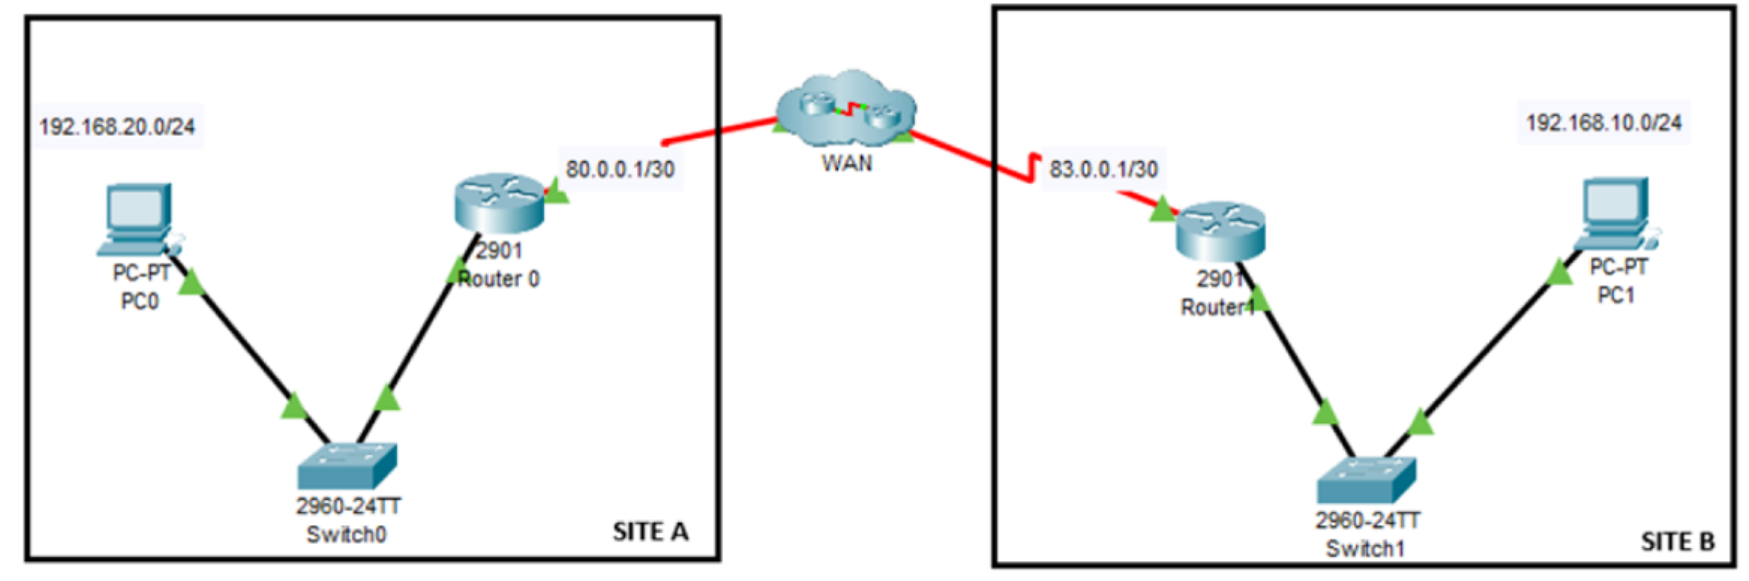
\includegraphics[width=0.8\textwidth]{contents/img/cisco_1.png}
\end{center}

\vspace{0.5cm}

Question~: Configurez les adresses IP pour chaque équipement et le NAT Overload. Utilisez les outils de diagnostic réseau (Ping,) pour vérifier l’accès de chaque poste client à Internet.

\vspace{0.5cm}

\begin{center}
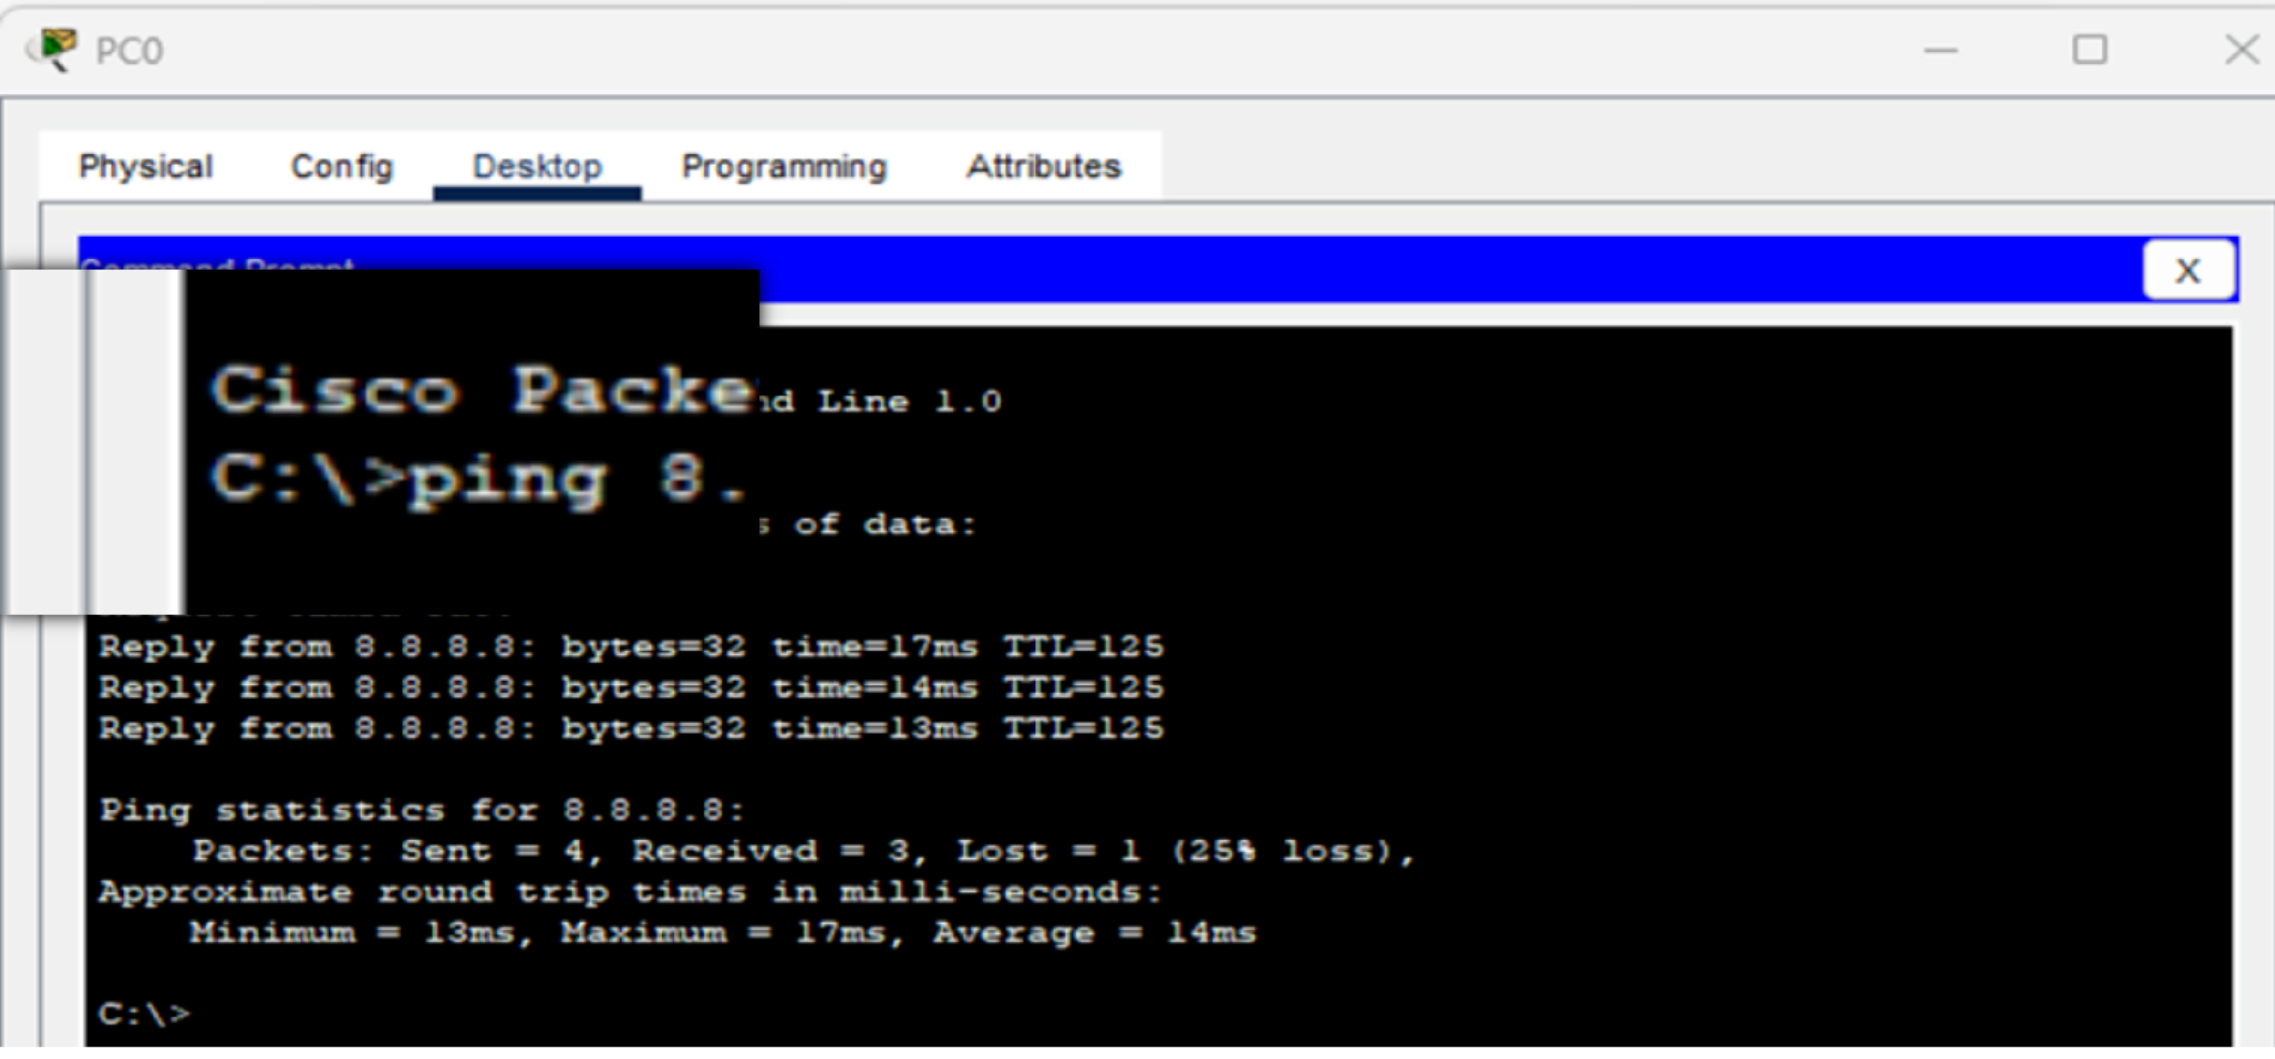
\includegraphics[width=0.7\textwidth]{contents/img/ping_google.png}
\end{center}

\begin{center}
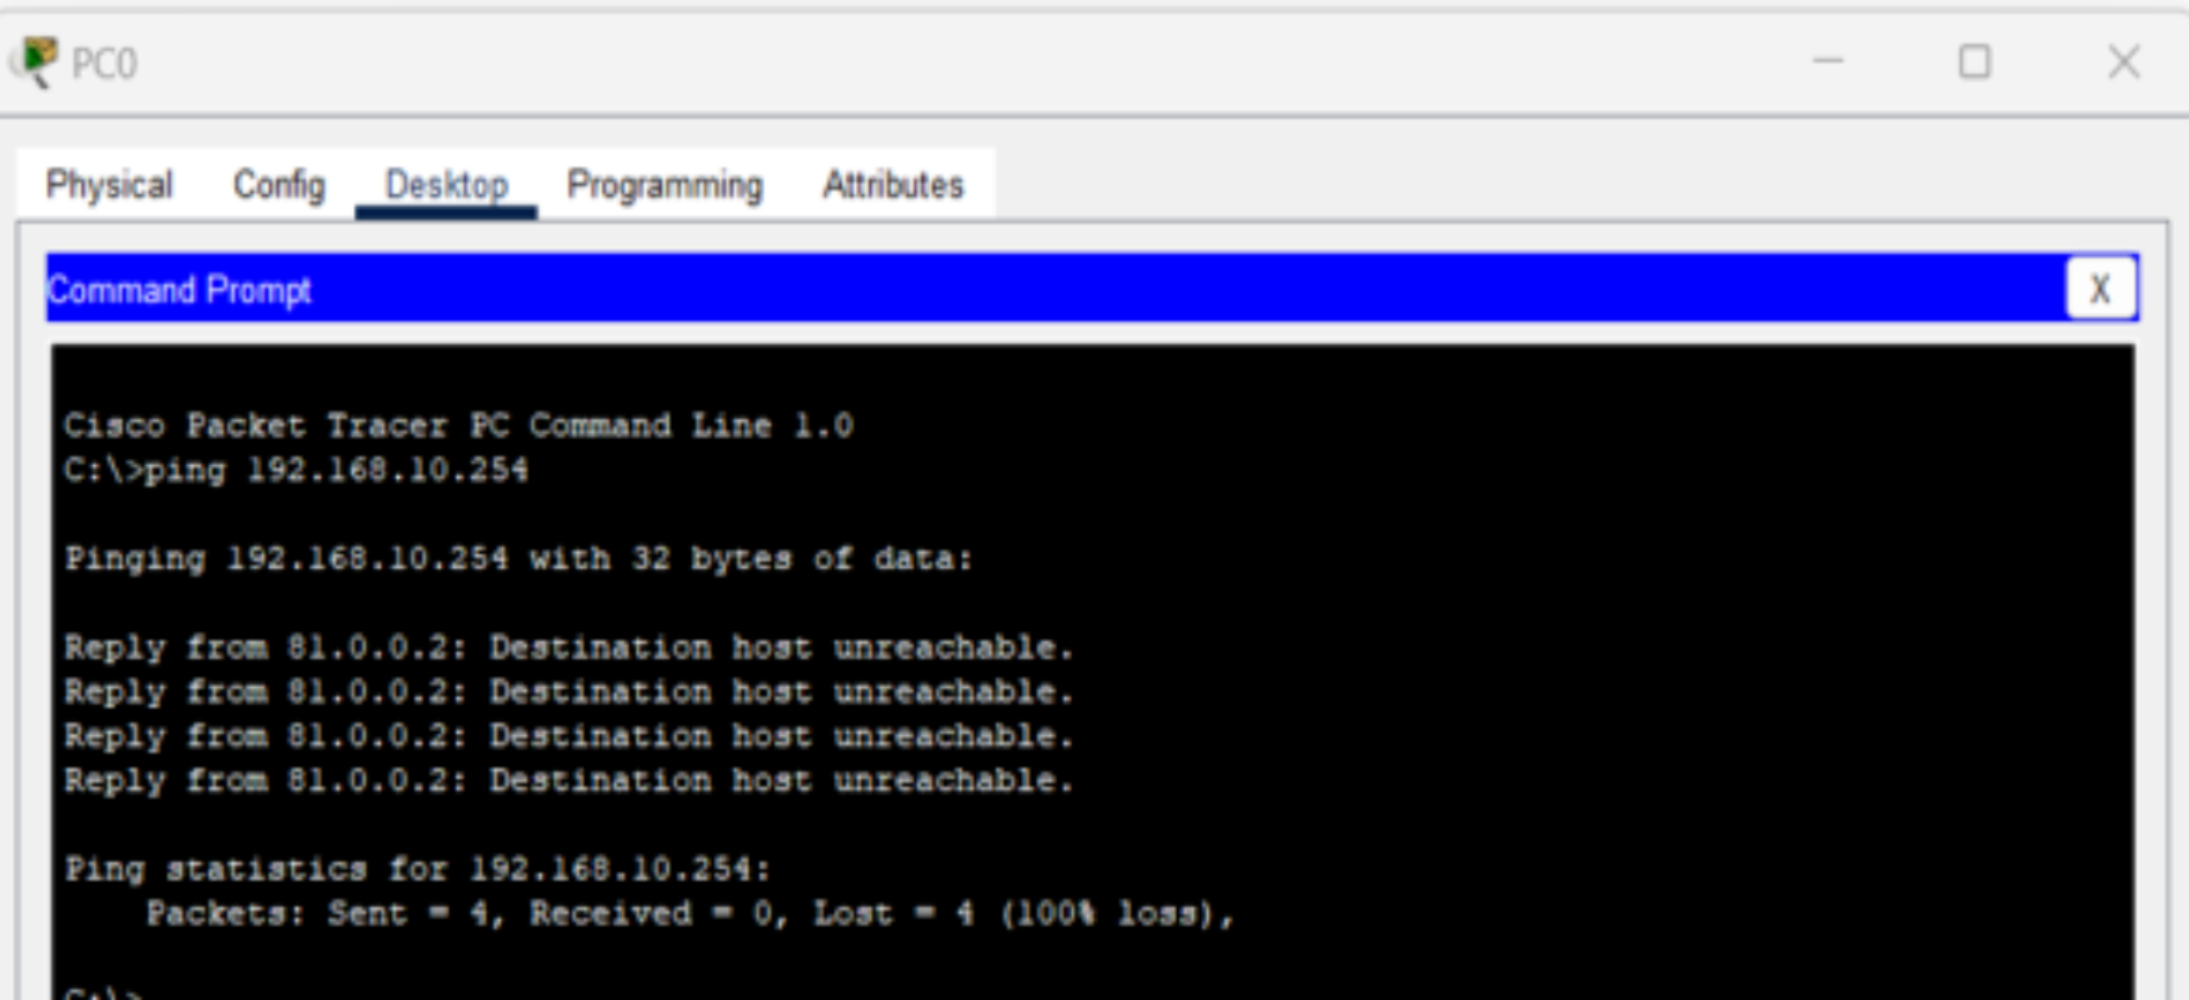
\includegraphics[width=0.7\textwidth]{contents/img/ping_ip.png}
\end{center}

\vspace{0.5cm}

\noindent Sous le nom de Translation d’Adresse Réseau, l’objectif du NAT est de changer une adresse IP par une autre.

\noindent NAT Overload, permet de traduire un nombre important d’IP du réseau local en une IP publique (ou plusieurs). Au contraire des NAT statiques et dynamiques dont le nombre de sessions simultanées se limitent au nombre d’IP publiques disponibles

\vspace{0.5cm}

Question~: Il faut activer le module de sécurité sur le routeur du site A. Comment activer le module sécurité securityk9 sur le routeur du site A ?

\vspace{0.5cm}

\noindent Exécutez la commande show version pour vérifier que la licence du pack est activée. Si ce n’est pas le cas, activez le module avec la commande suivante, enregistrez votre configuration et redémarrez votre routeur.

\begin{center}
  \begin{verbatim}
    SITEA>enable
    SITEA #conf t
    SITEA (config)#license boot module c2900 technology-package
    securityk9
    SITEA (config)#exit
    SITEA #copy run start
    SITEA #reload
  \end{verbatim}
\end{center}

\begin{center}
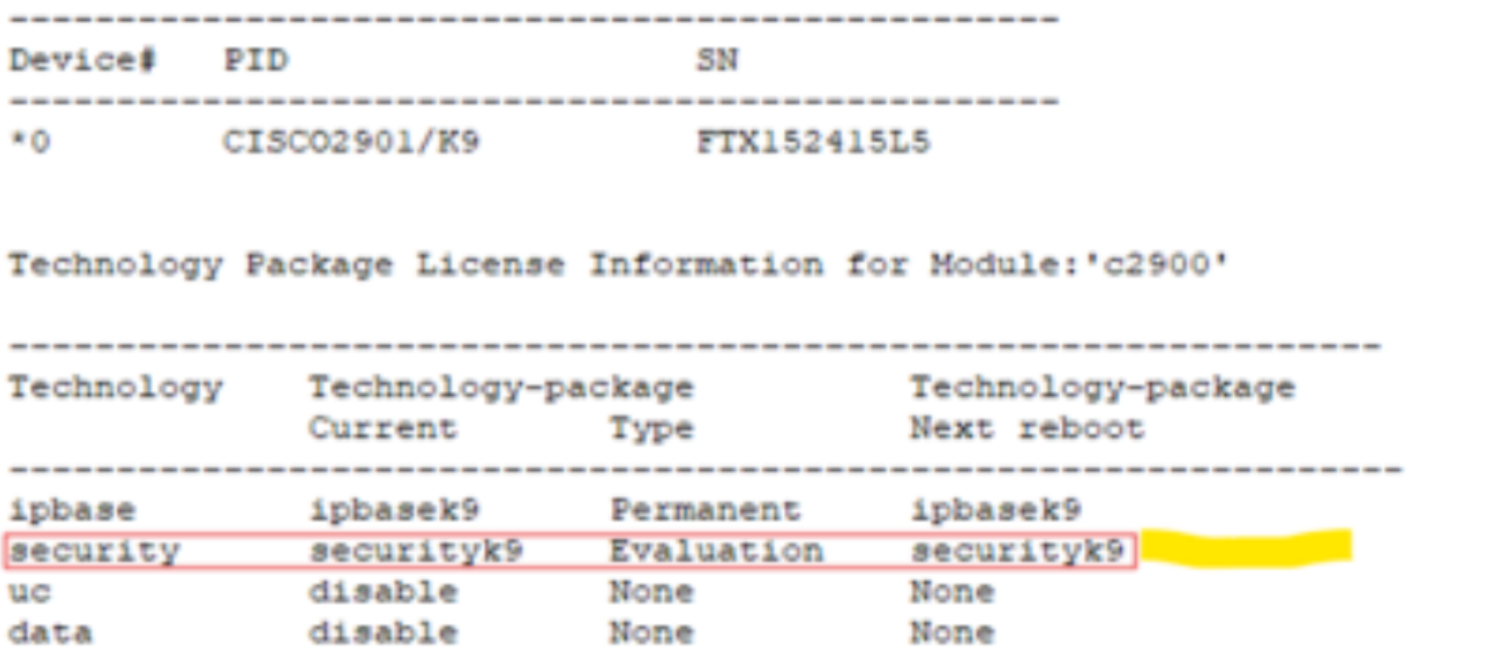
\includegraphics[width=0.8\textwidth]{contents/img/config_routeur.png}
\end{center}

\newpage

\noindent Le package technologique securityk9 comprend toutes les fonctionnalités de cryptographie, notamment IPsec, SSL/ SSH, Firewall et Secure VPN.

\vspace{0.5cm}

Question~: Configurer un VPN entre le site A et le site B de l’entreprise ADSNET et tester la connectivité en ces sites.

\vspace{0.5cm}

\noindent \textbf{ISAKMP}

\noindent Configuration du protocole de sécurité ISAKMP (Internet Security Association and Key Management Protocol). Il fournit la sécurisation des paquets qui seront acheminés d’un bout à l’autre.

\begin{center}
  \begin{verbatim}
    SITEA (config)#crypto isakmp policy 10
    SITEA (config-isakmp)# encryption aes
    SITEA (config-isakmp)# authentication pre-share
    SITEA (config-isakmp)# group 5
    SITEA (config-isakmp)#exit
  \end{verbatim}
\end{center}

\noindent Ce code configure les paramètres de base pour un VPN IPsec de type Site-to-Site, utilisant AES pour le chiffrement, une clé pré-partagée pour l'authentification, et le groupe Diffie-Hellman 5 pour l'échange de clés.

\begin{itemize}
  \item \textbf{encryption aes} : AES est le chiffrement choisi pour l’échange. Cet algorithme nécessite une clé pré-partagée pour le chiffrement et le déchiffrement (pre-share).
  \item \textbf{group 5} : Le group 5 représente l'algorithme DH (Diffie-Hellman) la manière selon laquelle une clé secrète partagée est établie entre les homologues.
  \item \textbf{crypto isakmp} : Crée une politique ISAKMP. Le protocole IKE est également appelé protocole ISAKMP (Internet Security Association and Key Management Protocol) (uniquement chez Cisco). IPsec utilise le protocole IKE pour négocier et établir des tunnels sécurisés de réseau privé virtuel (VPN) de site à site ou d’accès distant.
  \item \textbf{authentication pre-share} : Définit l'authentification par clé pré-partagée. Cette méthode signifie que les deux extrémités du VPN doivent avoir la même clé secrète configurée pour établir une connexion sécurisée.
\end{itemize}

\vspace{0.5cm}

\noindent \textbf{Le chiffrement AES}

\noindent Le chiffrement AES, ou norme de chiffrement avancée, est un chiffrement par bloc symétrique utilisé pour chiffrer les données sensibles. Avec une sécurité et une vitesse égales, AES est devenu une norme de sécurité pour les utilisateurs et les applications qui ont besoin d’un chiffrement facile à utiliser

\noindent AES-256 est la clé de chiffrement la plus puissante, mais son exécution nécessite beaucoup plus de puissance de traitement, de temps et de ressources qu’AES-128. Pour sécuriser les fichiers gouvernementaux top-secrets, AES-256 est le choix évident. Mais si l’objectif est de sécuriser une application sur un smartphone, par exemple, AES-128 peut être plus approprié

\noindent Même le niveau de cryptage AES le plus bas, AES-128, prendrait environ 1 milliard de milliards d’années pour se casser si vous utilisez une méthode de force brute.

\vspace{0.5cm}

\begin{center}
  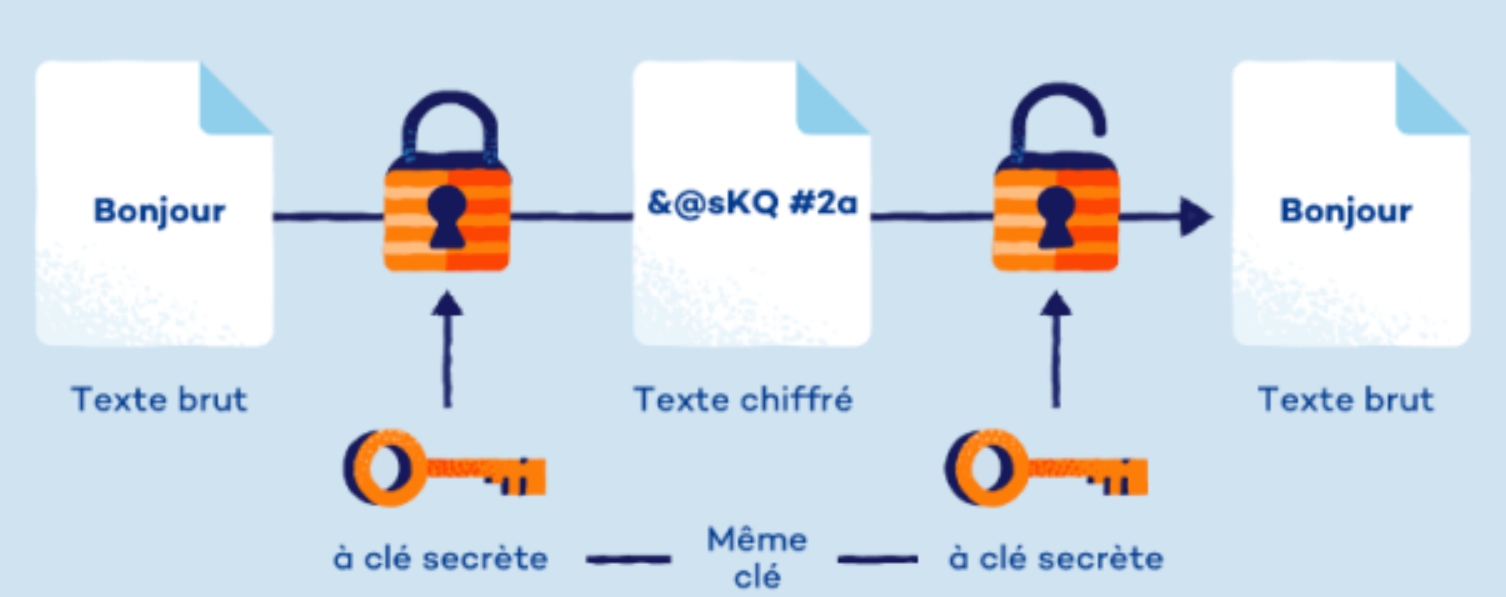
\includegraphics[width=0.8\textwidth]{contents/img/chiffrement_aes.png}
\end{center}

\vspace{0.5cm}

\noindent \textbf{IPsec}

\noindent IPsec est une suite de protocoles qui assure la sécurité des communications Internet au niveau de la couche IP. Il utilise des mécanismes de chiffrement et d'authentification pour protéger les données échangées entre deux points, garantissant ainsi la confidentialité, l'intégrité et l'authenticité des informations transmises.

\noindent L’utilisation actuelle la plus courante d’IPsec est de fournir un réseau privé virtuel (VPN), soit entre deux emplacements (passerelle à passerelle) ou entre un utilisateur distant et un réseau d’entreprise (hôte à passerelle). IPsec utilise le protocole IKE pour négocier et établir des tunnels sécurisés de réseau privé virtuel (VPN) de site à site ou d’accès distant.

\vspace{0.5cm}

Question~: Précisez la clé d’échange (KEYVPN) et la destination de l’hôte distant.

\begin{center}
  \begin{verbatim}
    SITEA (config)#crypto isakmp key KEYVPN address 83.0.0.1
  \end{verbatim}
\end{center}

\vspace{0.5cm}

Question~: Sélectionnez la méthode de cryptage que l’on appelle CRYPSET

\begin{center}
  \begin{verbatim}
    SITEA (config)#crypto ipsec transform-set CRYPSET esp-aes esp-sha-hmac
  \end{verbatim}
\end{center}

\noindent ESP-AES est l’algorythme de cryptage et esp-sha-hmac est la méthode d’authen-tification.

\vspace{0.5cm}

\noindent \textbf{Configuration des ACL :} 

\begin{center}
  \begin{verbatim}
    SITEA (config)#ip access-list extended LAN
    SITEA (config-ext-nacl)# no permit ip 192.168.20.0 
    0.0.0.255 any
    SITEA (config-ext-nacl)# deny ip 192.168.20.0 0.0.0.255 
    192.168.10.0 0.0.0.255
    SITEA (config-ext-nacl)# permit ip 192.168.20.0 0.0.0.255 any
    SITEA (config-ext-nacl)# exit
  \end{verbatim}
\end{center}

\vspace{0.5cm}

\noindent \textbf{Interdire la translation d’adresse vers le LAN distant}

\noindent L’ACL du NAT déjà existante qui s’appelle LAN est éditée dans le but d’interdire la translation d’adresse vers le LAN distant. De cette façon aucune adresse IP source à destination du site B ne sera changée. Néanmoins si la destination est autre que le site B, les adresses IP sources seront translatées.

\vspace{0.5cm}

\noindent \textbf{ACL}

\noindent La notion d'ACL est dit assez généraliste, et on peut parler d'ACL pour gérer les accès à n'importe quel type de ressource. Il existe deux types d’ACL de base :

\begin{itemize}
  \item \textbf{ACL de système de fichiers:} Ils fonctionnent comme des filtres, gérant l’accès aux annuaires ou aux fichiers. Un ACL de système de fichiers donne des instructions au système d’exploitation sur les utilisateurs autorisés à accéder au système, ainsi que sur les privilèges auxquels ils ont droit une fois qu’ils sont à l’intérieur.
  \item \textbf{ACL réseau:} Les ACL réseau gèrent l’accès à un réseau. Pour ce faire, ils fournissent des instructions aux commutateurs et routeurs quant aux types de trafic qui sont autorisés à s’interfacer avec le réseau. Ils dictent également ce que chaque utilisateur ou appareil peut faire une fois qu’il est à l’intérieur.
\end{itemize}

\noindent Une ACL sur un pare-feu ou un routeur filtrant, est une liste d'adresses ou de ports autorisés ou interdits par le
dispositif de filtrage.

\noindent Les Access Control List sont divisés en trois grandes catégories, l'ACL standard, l'ACL étendue et la nommée-
étendue.

\begin{itemize}
  \item L'ACL standard ne peut contrôler que deux ensembles : l'adresse IP source et une partie de l'adresse IP de destination, au moyen de masque générique.
  \item L'ACL étendue peut contrôler l'adresse IP de destination, la partie de l'adresse de destination (masque générique), le type de protocole (TCP, UDP, ICMP, IGRP, IGMP, etc.), le port source et de destination, les flux TCP, IP TOS (Type of service) ainsi que les priorités IP.
  \item L'ACL nommée-étendue est une ACL étendue à laquelle on a affecté un nom.
\end{itemize}

\vspace{0.5cm}

\noindent \textbf{ACL VPN}

\noindent Créez une autorisation qui autorise le réseau du site A à communiquer avec le réseau du site B avec l’ACL que qu’on nommera « VPN ».

\vspace{0.5cm}

\begin{center}
  \begin{verbatim}
    SITEA (config)#ip access-list extended VPN
    SITEA (config-ext-nacl)# permit ip 192.168.20.0 0.0.0.255
    192.168.10.0 0.0.0.255
  \end{verbatim}
\end{center}

\newpage

\noindent Regroupez les éléments créés précédemment pour en faire une cryptomap qui sera positionnée sur l’interface Outside serial 0/0/0

\vspace{0.5cm}

\begin{center}
  \begin{verbatim}
    SITEA (config)#crypto map VPNMAP 10 ipsec-isakmp
    SITEA (config-crypto-map)# set peer 83.0.0.1
    SITEA (config-crypto-map)# set transform-set CRYPSET
    SITEA (config-crypto-map)# match address VPN
    SITEA (config-crypto-map)#exit
    SITEA (config)#interface serial 0/0/0
    SITEA (config-if)#crypto map VPNMAP
    *Jul 11 15:33:05.785: %CRYPTO-6-ISAKMP_ON_OFF: ISAKMP is ON
  \end{verbatim}
\end{center}

\vspace{0.5cm}

\begin{center}
  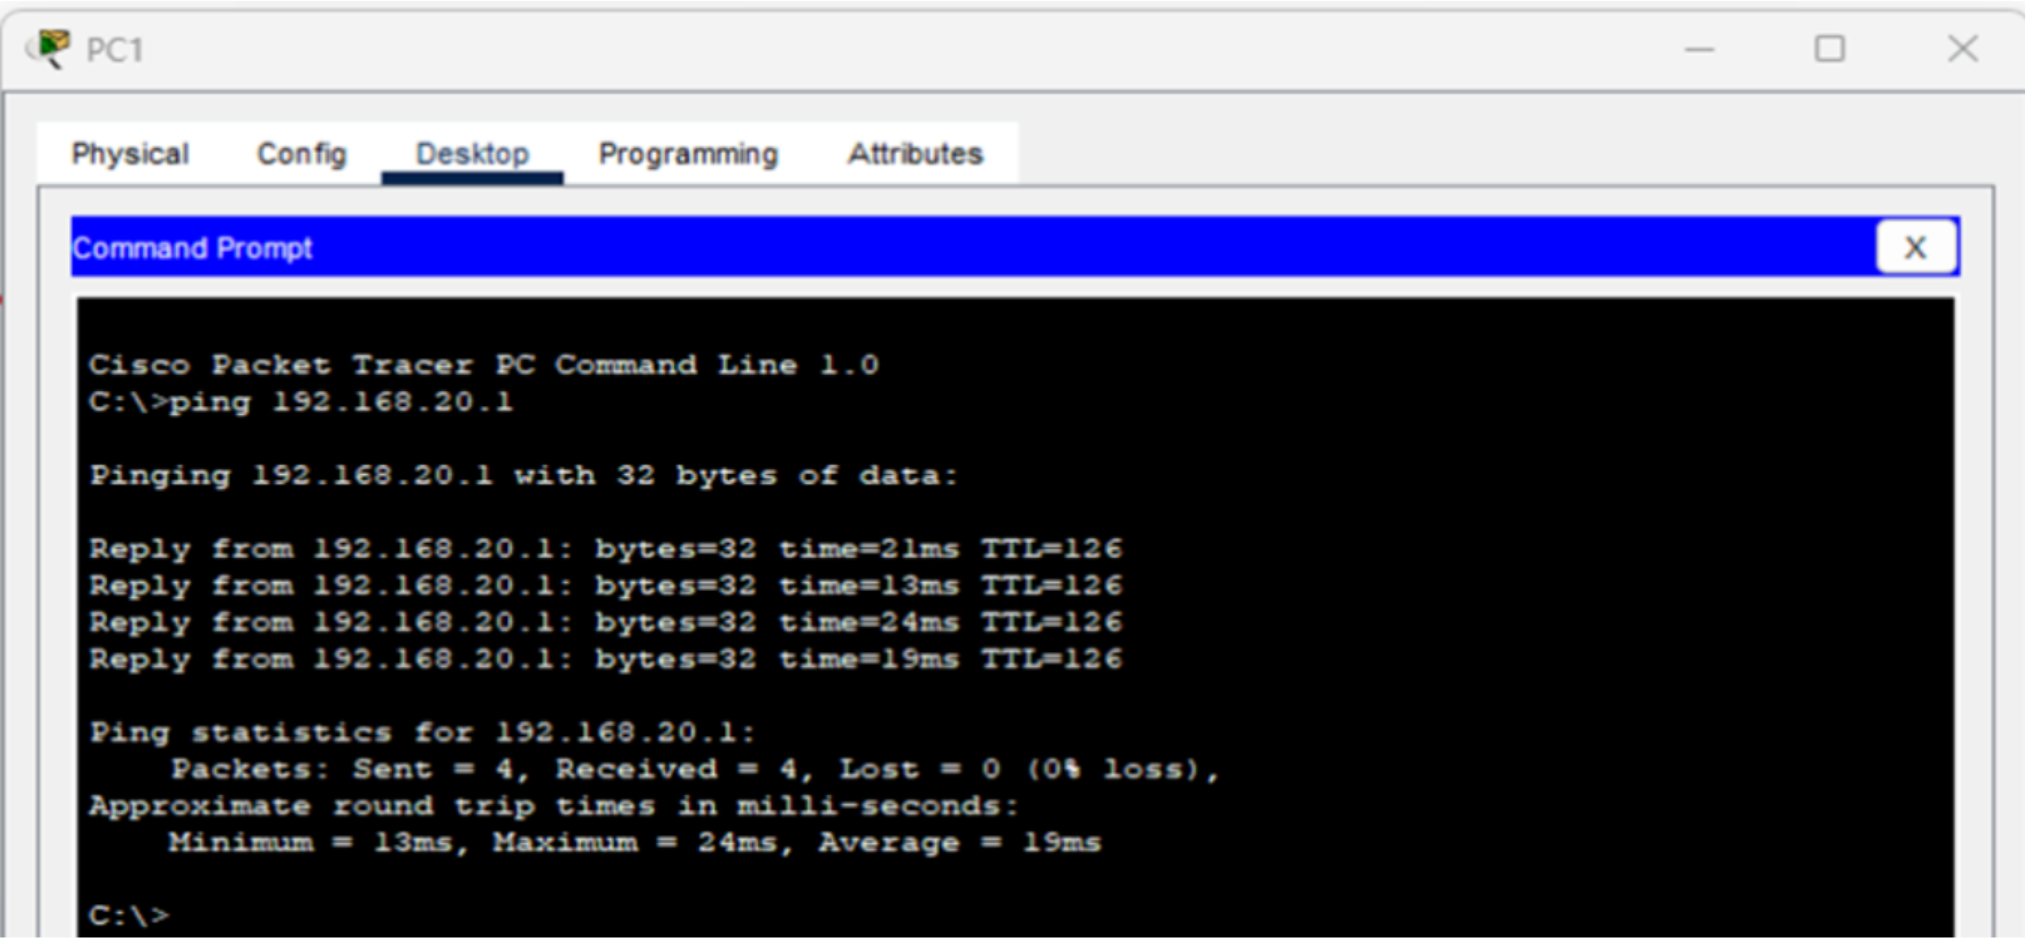
\includegraphics[width=0.8\textwidth]{contents/img/ping_reussi.png}
\end{center}

\vspace{0.5cm}

\noindent On effectue les mêmes configurations sur le routeur du site B. Faire un test de connectivité entre les deux sites.

\noindent Effectuer un Ping à partir du poste client d’un des sites A ou B vers un poste client d’un site externe A ou B

\vspace{0.5cm}

Question~: Vérifiez si l’échange de paquets entre les deux hôtes est crypté.

\begin{center}
  \begin{verbatim}
    SITEA #show crypto ipsec sa
  \end{verbatim}
\end{center}

\newpage

\subsection*{Installation d'un serveur VPN Client to Site}
\phantomsection
\addcontentsline{toc}{subsection}{Installation d'un serveur VPN Client to Site}

\noindent L’entreprise ADSNET souhaite permettre l'accès à son réseau local aux utilisateurs en télétravail à travers un lien sécurisé (VPN).

\noindent Elle utilise un pare-feu pfSense et souhaite l'utiliser pour mettre en place un accès VPN.

\vspace{0.5cm}

Question~: Comment s'appelle ce type d'accès VPN ?

\vspace{0.5cm}

\noindent \textbf{VPN client-to-site}

\noindent Lorsqu’un tunnel VPN est établi entre un appareil (ordinateur, smartphone, tablette, etc.) et un réseau d’entreprise, on parle de VPN client-to-site. Ce type de VPN est idéal pour le télétravail ou les déplacements, permettant aux utilisateurs de se connecter de manière sécurisée au réseau de leur entreprise depuis des endroits tels que leur domicile, un hôtel, un restaurant, ou encore en rendez-vous chez un client.

\noindent La possibilité que plusieurs employés se connectent de manière sécurisée au réseau d’entreprise à distance via un VPN client-to-site avec une connexion sécurisée, offre un accès aux données sur le serveur de fichiers ou à des applications hébergées sur un serveur, garantissant la confidentialité des informations. Contrairement à d’autres outils de connexion à distance, le VPN est privilégié pour sa sécurité accrue.

\vspace{0.5cm}

Question~: Quelles sont les options VPN Client-To-Site proposées par pfSense ?

\vspace{0.5cm}

\begin{center}
  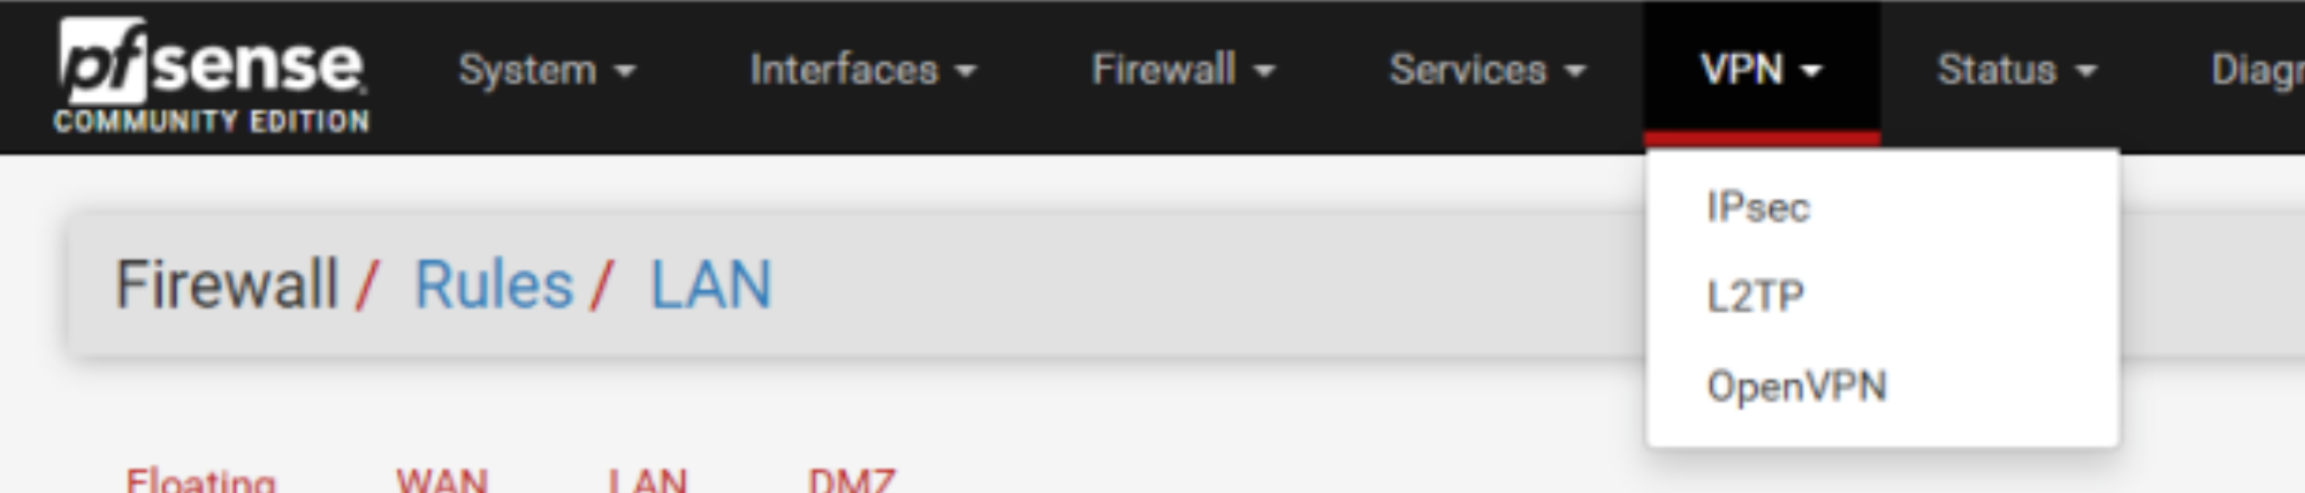
\includegraphics[width=0.8\textwidth]{contents/img/pfsense.png}
\end{center}

\newpage

\noindent \textbf{Options VPN de pfSense}

\noindent Le logiciel pfSense propose plusieurs options VPN : IPsec, OpenVPN, WireGuard et L2TP.

\vspace{0.5cm}

\begin{center}
  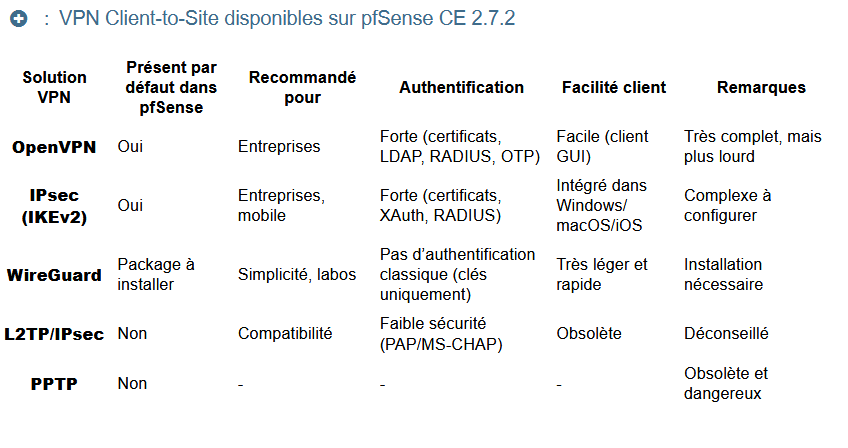
\includegraphics[width=1\textwidth]{contents/img/option_pfsense.png}
\end{center}

\vspace{0.5cm}

Question~: Qu'est-ce que Wireguard ?

\vspace{0.5cm}

\noindent \textbf{WireGuard}

\noindent WireGuard est un protocole VPN qui vise à remplacer IKEv2/IPSec et OpenVPN grâce à une conception moderne.

\noindent Il utilise des algorithmes cryptographiques de dernière génération :

\begin{itemize}
  \item Curve25519 (échange de clés)
  \item ChaCha20 (chiffrement)
  \item Poly1305 (authentification)
\end{itemize}

\noindent Son code source très réduit (~4000 lignes), ce qui limite les bugs et facilite l’audit. WireGuard ne gère pas l'authentification au sens classique (login/mot de passe, certificats ou MFA).

\noindent Il repose uniquement sur des clés cryptographiques (clé publique/clé privée). Il faut donc générer une paire de clés pour chaque client.

\vspace{0.5cm}

\newpage

Question~: Quelle plateforme peut-on utiliser pour mettre en place un serveur VPN WireGuard ?

\noindent \textbf{Ubuntu, Debian, CentOS, Fedora, Arch Linux, etc.}

\noindent Il est possible d'utiliser les solutions suivantes pour déployer WireGuard :

\begin{itemize}
  \item Serveur Linux (le plus courant) comme Ubuntu, Debian, CentOS, Fedora, Arch Linux, etc.
  \item Facile à installer : apt install wireguard, dnf install wireguard-tools , etc.
  \item WireGuard est intégré directement au noyau Linux à partir de la version 5.6, ce qui signifie que le support est maintenu et optimisé nativement par le noyau lui-même.
  \item Appliances et pare-feu avec support WireGuard (exemple : pfSense).
  \item Services Cloud.
\end{itemize}

\subsection*{VPN Client-To-Site avec pfSense et Wiregard}
\phantomsection
\addcontentsline{toc}{subsection}{VPN Client-To-Site avec pfSense et Wiregard}

\noindent Vous choisissez finalement d'installer un VPN Client-To-Site avec pfSense et Wireguard avec un client WireGuard sur les PC des
utilisateurs en télétravail.

\noindent Vous allez faire une maquette en utilisant votre PC et VMWare Pro.

\vspace{0.5cm}

\begin{center}
  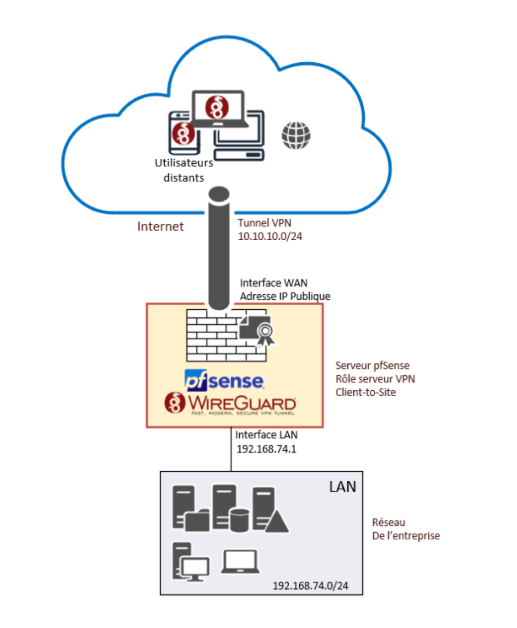
\includegraphics[width=0.5\textwidth]{contents/img/architecture_wiregard_pfsense.png}
\end{center}

\vspace{0.5cm}

\begin{center}
  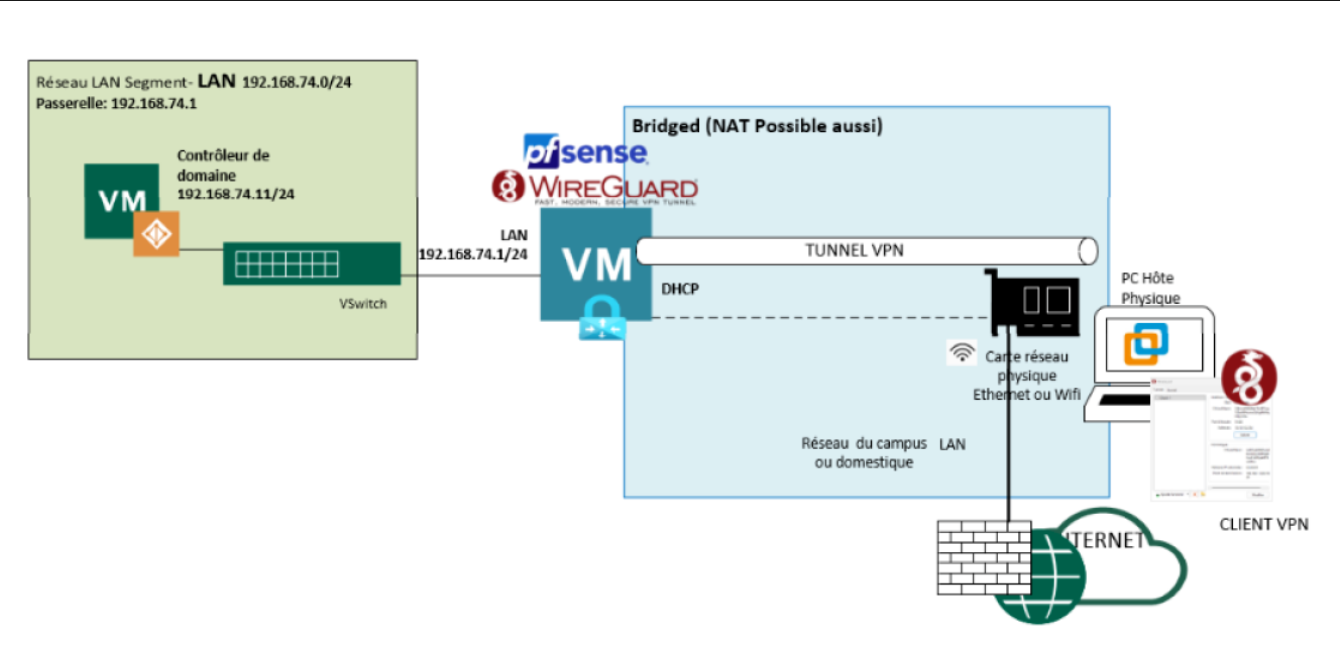
\includegraphics[width=0.7\textwidth]{contents/img/architecture_vm.png}
\end{center}

\vspace{0.5cm}

\noindent Voici l'architecture de votre maquette nécessaire à cette partie de la corbeille.

\vspace{0.5cm}

\noindent Vous avez besoin de votre PC avec VMWare Workstation Pro et :

\begin{itemize}
  \item D'une \textbf{VM pfSense} avec deux interface réseau, une sur un réseau \textbf{LAN Segment:LAN} et une en mode \textbf{Bridged}.
  \item Vous avez besoin d'un serveur Windows avec une interface dans le réseau \textbf{LAN Segment:LAN} qui vous servira pour tester l'accès distant à un serveur.
\end{itemize}

\vspace{0.5cm}

\noindent Vous n'êtes pas obligé d'utiliser une VM contrôleur de domaine sauf si vous utilisez une VM pfSense utilisant des l'annuaire LDAP.

\noindent Le client VPN sera installé sur votre PC physique et c'est votre PC physique qui va initier la connexion au serveur VPN et accéder au serveur Windows dans le LAN (d'où le mode bridged).

\noindent Si votre VM pfSense a une interface DMZ, ce n'est pas grave.

\subsection*{Installation de WireGuard sur pfSense}
\phantomsection
\addcontentsline{toc}{subsection}{Installation de WireGuard sur pfSense}

\noindent L'installation se fait en plusieurs plusieurs étapes mais est très rapide.
\begin{itemize}
  \item Installation du package WireGuard.
  \item Ajout et configuration du tunnel VPN.
  \item Activation du service VPN.
  \item Configuration de l'interface VPN.
  \item Configuration du client VPN et ajout et configuration du pair.
  \item Ajout et configuration des règles de pare-feu.
  \item Tests
\end{itemize}

\vspace{0.5cm}

Questions~: Qu'est-ce qu'un réseau P2P (peer-to-peer) ? Quel rapport avec WireGuard ?

\vspace{0.5cm}

\noindent \textbf{P2P}

\noindent Le \textbf{P2P} est un modèle dans lequel chaque ordinateur joue un rôle \textbf{égalitaire} dans le réseau : il peut \textbf{recevoir et envoyer} des données à d’autres sans passer par un serveur central.

\vspace{0.5cm}

\noindent \textbf{Fonctionnement P2P de WireGuard}

\noindent Fonctionnement P2P de WireGuard

\begin{itemize}
  \item Les deux machines \textbf{s'authentifient mutuellement} via leur \textbf{clé publique}
  \item L’un des peers initie la connexion, mais ensuite \textbf{la communication est bidirectionnelle}
  \item Pas besoin d’un serveur central pour faire transiter le trafic
\end{itemize}
\noindent Résultat : \textbf{WireGuard fonctionne comme un vrai protocole peer-to-peer chiffré.}

\vspace{0.5cm}

\noindent \textbf{Attention}

\noindent Dans pfSense, le tunnel WireGuard n'est ni strictement client ni strictement serveur.

\noindent C’est un peer parmi d'autres, comme l’exige le modèle P2P de WireGuard. Cependant lors de sa configuration on lui attribue un rôle fonctionnel. Dans le cadre de cette corbeille pfSense sera un serveur passif en attente que le client se connecte.

\noindent \textbf{Rôles fonctionnels de WireGuard dans pfSense}

\vspace{0.5cm}

\begin{center}
\setlength{\tabcolsep}{12pt}
\begin{tabular}{|p{0.25\textwidth}|p{0.55\textwidth}|}
\hline
\textbf{Rôle fonctionnel} & \textbf{Description} \\ \hline

Serveur (passif) & pfSense attend que le peer se connecte (port UDP ouvert) \\ \hline

Client (actif) & pfSense initie la connexion vers un peer distant \\ \hline

Site-à-site & pfSense <-> pfSense ou routeur WireGuard <-> WireGuard \\ \hline

\end{tabular}
\end{center}

\vspace{0.5cm}

\noindent \textbf{Technologies P2P}

\noindent Exemples de technologies P2P

\begin{itemize}
  \item BitTorrent : partage de fichiers
  \item Skype (anciennement) : appels audio/vidéo
  \item Blockchain (Bitcoin, Ethereum) : registre distribué
  \item IPFS : système de fichiers distribué
\end{itemize}

\vspace{0.5cm}

Question~: Comment installer le \textbf{package WireGuard} sous pfSense ? une idée ?

\vspace{0.5cm}

\noindent \textbf{PfSense et WireGuard}

\noindent Pour rappel, pfsense est un routeur/pare-feu open source basé sur le système d’exploi-tation FreeBSD. La version gratuite est la version CE.

\noindent Netgate supporte WireGuard dans pfSense à partir de la version 2.7.0+ (2023) via plugin.

\noindent pfSense Plus 23.01 l'intègre et le maintient officiellement.

\vspace{0.5cm}

\begin{center}
  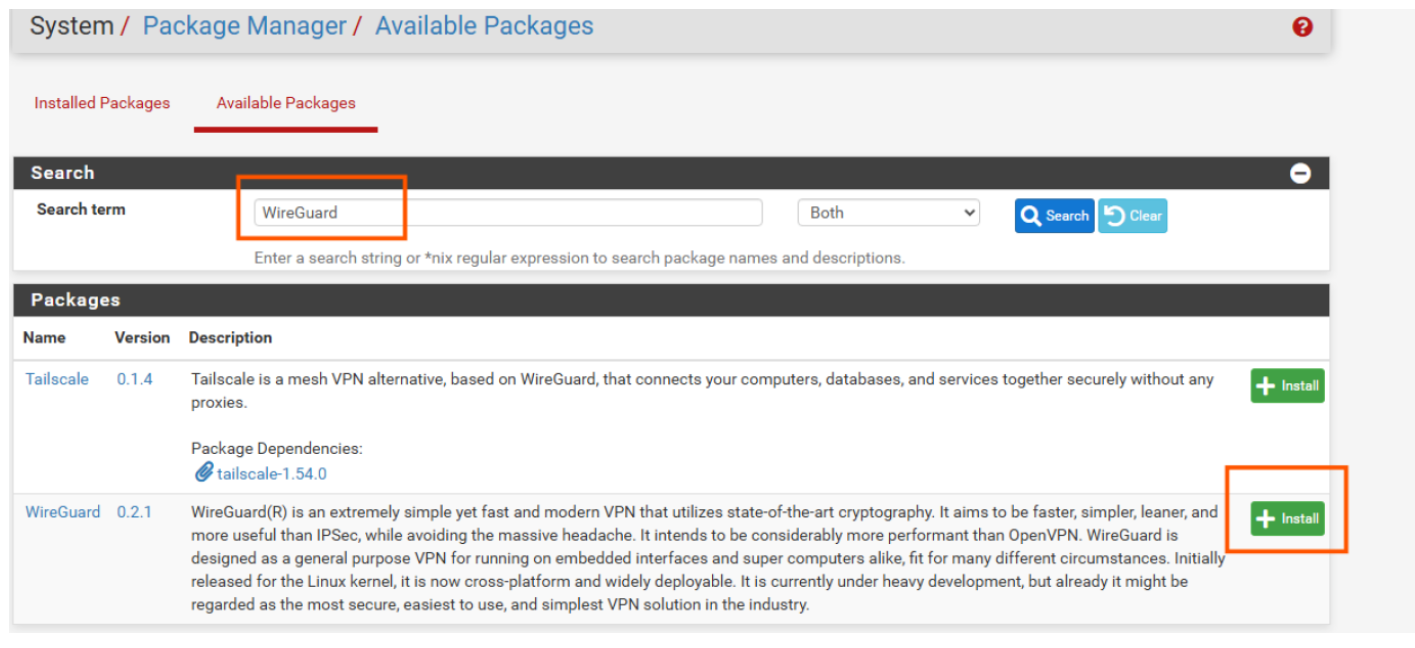
\includegraphics[width=0.8\textwidth]{contents/img/install_wiregard_pfsense.png}
\end{center}

\vspace{0.5cm}

\begin{itemize}
  \item Connectez-vous à l’interface web pfSense avec un accès administrateur.
  \item \textbf{System > Package Manager > Available Packages}.
  \item Chercher \textbf{WireGuard} et cliquer sur \textbf{Install} puis \textbf{Confirm}.
  \item Attendre la fin de l’installation
\end{itemize}

\vspace{0.5cm}

\begin{center}
  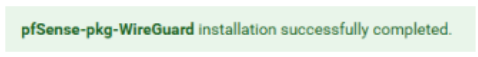
\includegraphics[width=0.8\textwidth]{contents/img/pfsense_success.png}
\end{center}

\newpage

\subsection*{Configuration de WireGard}
\phantomsection
\addcontentsline{toc}{subsection}{Configuration de WireGard}

\noindent Vous avez installé le package, maintenant il est nécessaire de configurer le tunnel VPN. Votre administrateur réseau vous demande d'utiliser le réseau 10.10.10.0/24 pour votre tunnel VPN.

\noindent Vous allez :

\begin{itemize}
  \item Ajouter et configurer un tunnel VPN
  \item Activer WireGuard et configurer l'interface associée
\end{itemize}

\noindent Pour configurer le tunnel VPN vous devez renseigner une description (par exemple Remote VPN-USERS), vous devez avoir l'adresse assignée à l'interface, ici 10.10.10.1/24. Cette adresse doit être dans un réseau IP différent que le réseau WAN et le LAN. Vous devez définir le port d'écoute (par défaut port UDP 51820).

\noindent Vous avez la possibilité de générer la clé publique et la clé privée.

\vspace{0.5cm}

\begin{center}
  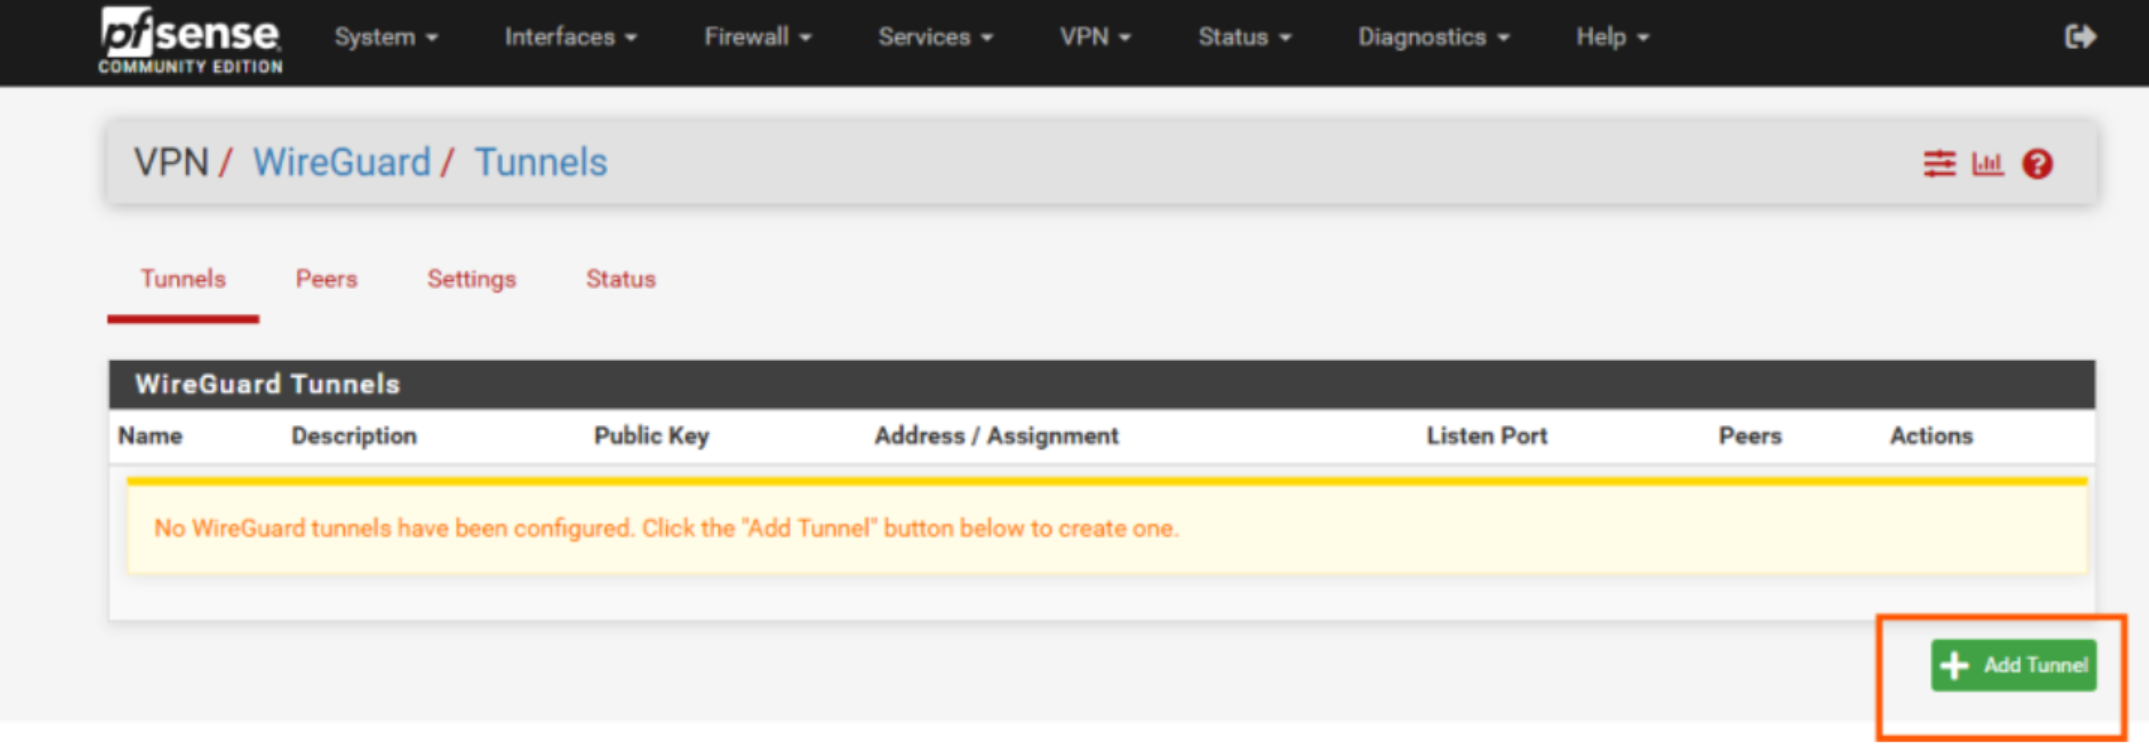
\includegraphics[width=0.8\textwidth]{contents/img/wireguard.png}
\end{center}

\begin{itemize}
  \item Vous allez utiliser le menu VPN > WireGuard.
  \item Cliquez sur + Add Tunnel pour créer un nouveau tunnel.
\end{itemize}

\vspace{0.5cm}

\begin{center}
  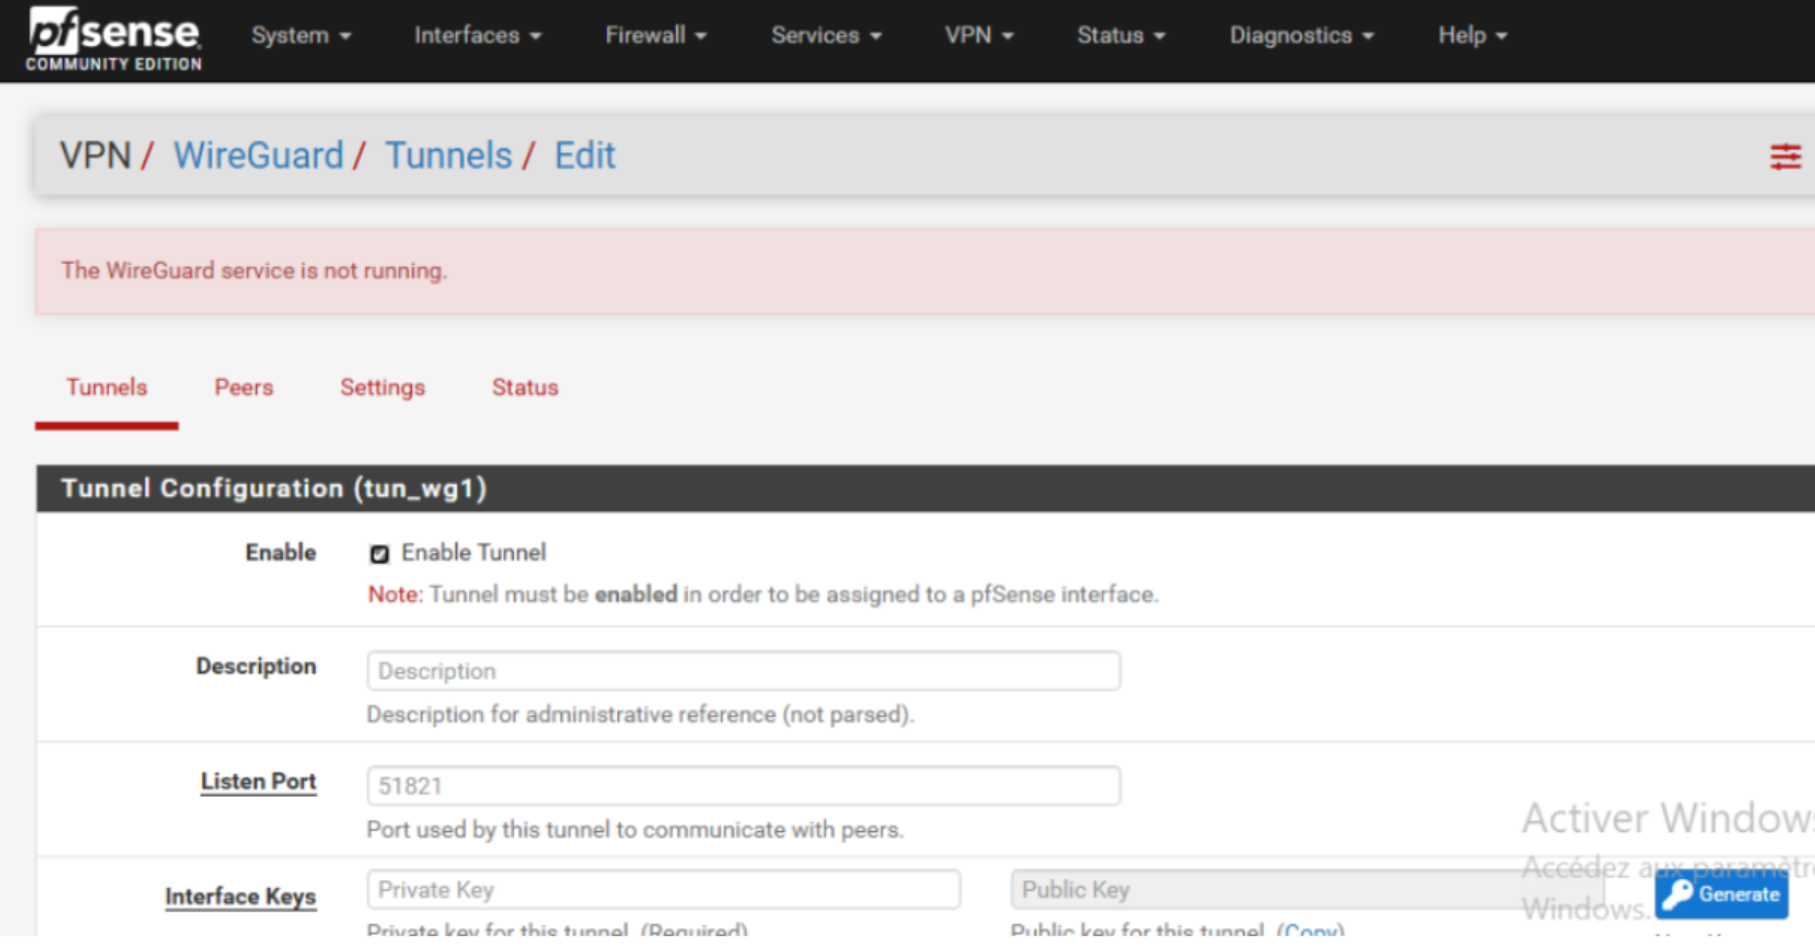
\includegraphics[width=0.8\textwidth]{contents/img/wireguard_config.png}
\end{center}

\newpage

\noindent Configure le tunnel :

\begin{itemize}
  \item Cochez Enabled
  \item Description : VPN-USERS (indiquez une description)
  \item Interface Address : 10.10.10.1/24 Adresse IP du Tunnel VPN au format CIDR. \\ Cette adresse doit être dans un réseau IP différent que WAN et LAN
  \item Listen Port : 51820 (par défaut port UDP 51820)
  \item Dans Interface Keys, cliquez sur Generate
  \item Copiez la clé publique du tunnel en cliquant sur (Copy).
  \item Cliquez sur Save pour enregistrer la configuration du tunnel VPN
\end{itemize}

\vspace{0.5cm}

\begin{center}
  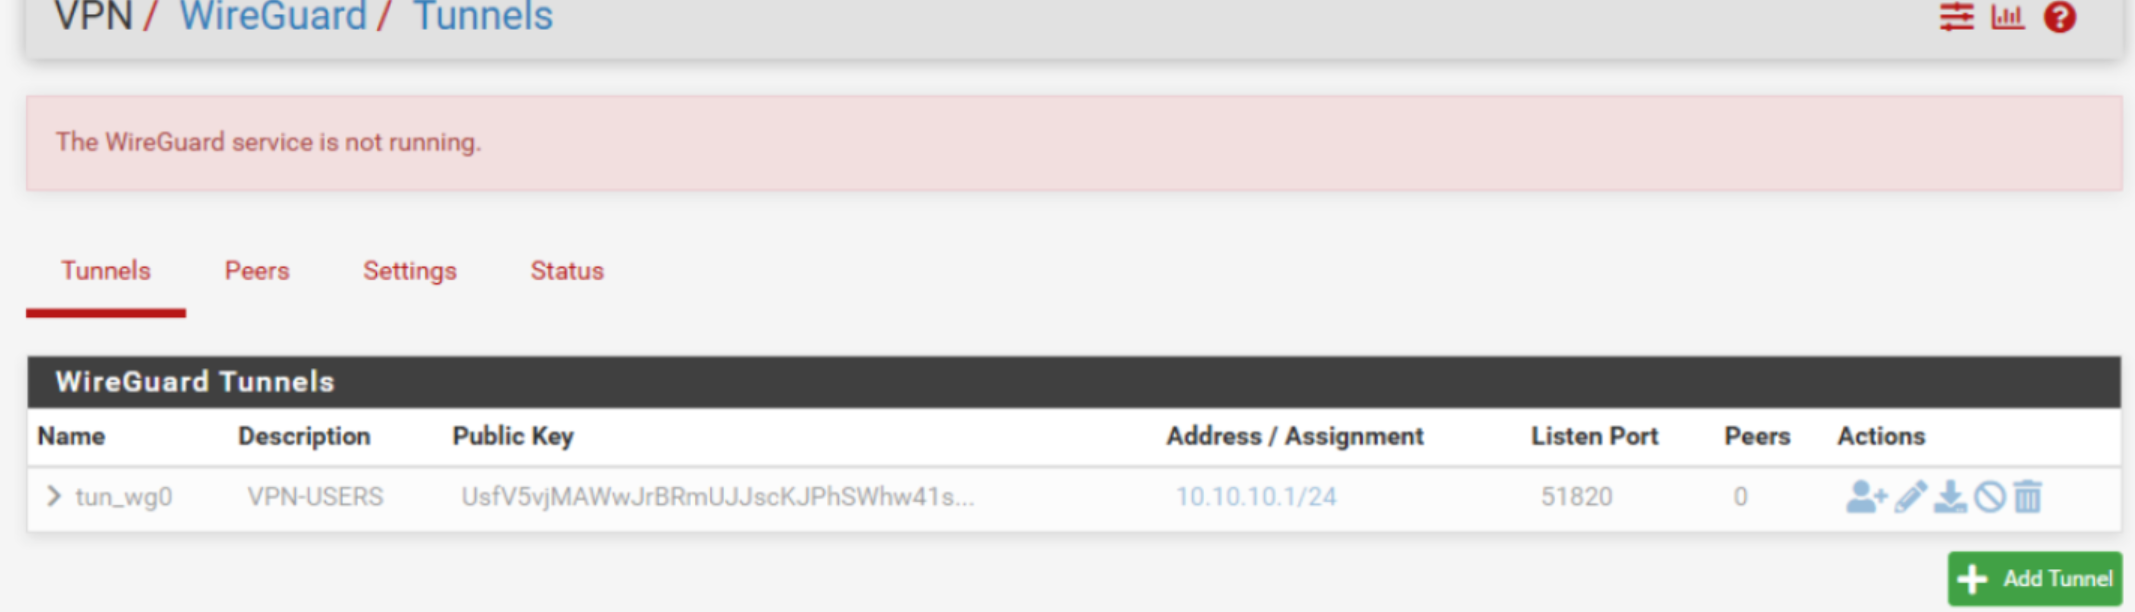
\includegraphics[width=0.8\textwidth]{contents/img/wireguard_save.png}
\end{center}

\noindent Vous allez avoir besoin de la clé publique du tunnel pour paramétrer les clients VPN, copiez-la et enregistrez-la.

\vspace{0.5cm}

Question~: Quel algorithme est utilisé pour générer les clés ?

\vspace{0.5cm}

\noindent WireGuard utilise la cryptographie à courbe elliptique (Curve25519).

\begin{itemize}
  \item La clé privée est une valeur aléatoire de 256 bits
  \item La clé publique est dérivée de la clé privée par une opération mathématique sécurisée
\end{itemize}

\noindent D'un point de vue cryptographique, Wireguard utilise :

\begin{itemize}
  \item Curve25519 pour l'échange de clé
  \item ChaCha20 pour la cryptographie symétrique
  \item Poly1305 pour le code d'authentification de message
  \item SipHash pour les tables de hachage
  \item BLAKE2s pour les fonctions de hachage
  \item UDP pour des échanges plus rapides
\end{itemize}

\newpage

Question~: Pourquoi utiliser ce réseau 10.10.10.0/24 et une adresse pour l'interface ?

\vspace{0.5cm}

\noindent \textbf{Réseau IP dédié au tunnel}

\noindent Un réseau IP est associé à un tunnel VPN pour créer une connexion privée et sécurisée entre deux réseaux ou machines distants, comme s’ils étaient sur un même réseau local. Voici les raisons principales de cette association :

\noindent Le VPN crée un tunnel crypté dans lequel transitent les paquets IP.

\noindent Le réseau IP assigné au tunnel (ex. 10.10.10.0/24) est virtuel et n’existe que dans le VPN. Cela empêche toute fuite vers Internet en clair.

\noindent Exemple : Le client VPN reçoit une IP comme 10.10.10.2, et cette IP est utilisée uniquement à l’intérieur du tunnel VPN pour communiquer avec le serveur 10.10.10.1.

\vspace{0.5cm}

\noindent \textbf{Pourquoi un réseau IP dédié au tunnel}

\noindent Associer un réseau IP dédié au tunnel permet de :

\begin{itemize}
  \item Ajouter facilement des routes
  \item Séparer le trafic VPN du trafic normal
  \item Gérer les ACL, les pare-feu, les QoS ou les logs
  \item Faciliter la gestion réseau et l’interconnexion de sites
\end{itemize}

\noindent Cela va vous permettre d’identifier si une machine est connectée via VPN en regardant son IP.

\newpage

\subsection*{Configuration de l'interface associée au tunnel}
\phantomsection
\addcontentsline{toc}{subsection}{Configuration de l'interface associée au tunnel}

\noindent L'installation du tunnel WireGuard implique de configurer une nouvelle interface virtuelle qui lui est associé et que vous pouvez voir dans le menu Interfaces/Interface Assignments

\noindent Vous allez voir une nouvelle interface OPT associée à tun\_wg0 (tun\_wg0)

\noindent Il suffit de lui affecter l'adresse IP associée au tunnel.

\vspace{0.5cm}

\begin{center}
  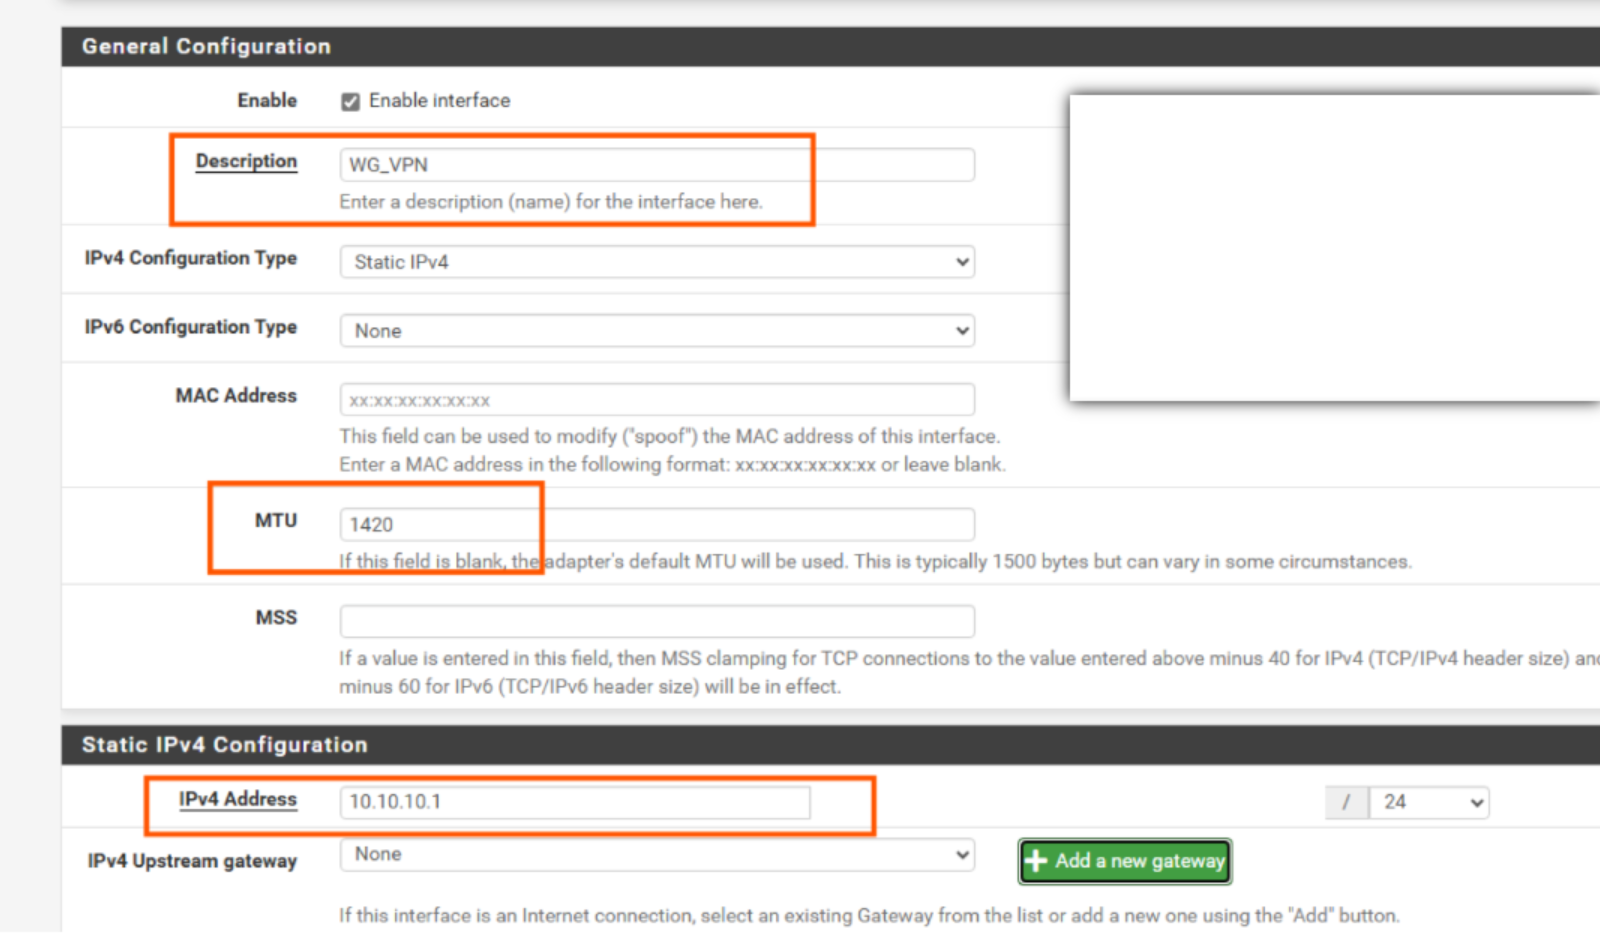
\includegraphics[width=0.8\textwidth]{contents/img/interface_wg.png}
\end{center}

\vspace{0.5cm}

\begin{itemize}
  \item Activez l'interface avec Enable interface
  \item Donnez lui une description (ici par exemple WG\_VPN)
  \item IPv4 Configuration Type : Static IPv4
  \item IPv4 Address : Indiquez l'adresse IP affectée au tunnel ici 10.10.10.1/24
  \item Fixez le MTU à 1420 (en contexte VPN)
  \item Cliquez sur Save et sur Apply
\end{itemize}

\vspace{0.5cm}

\begin{center}
  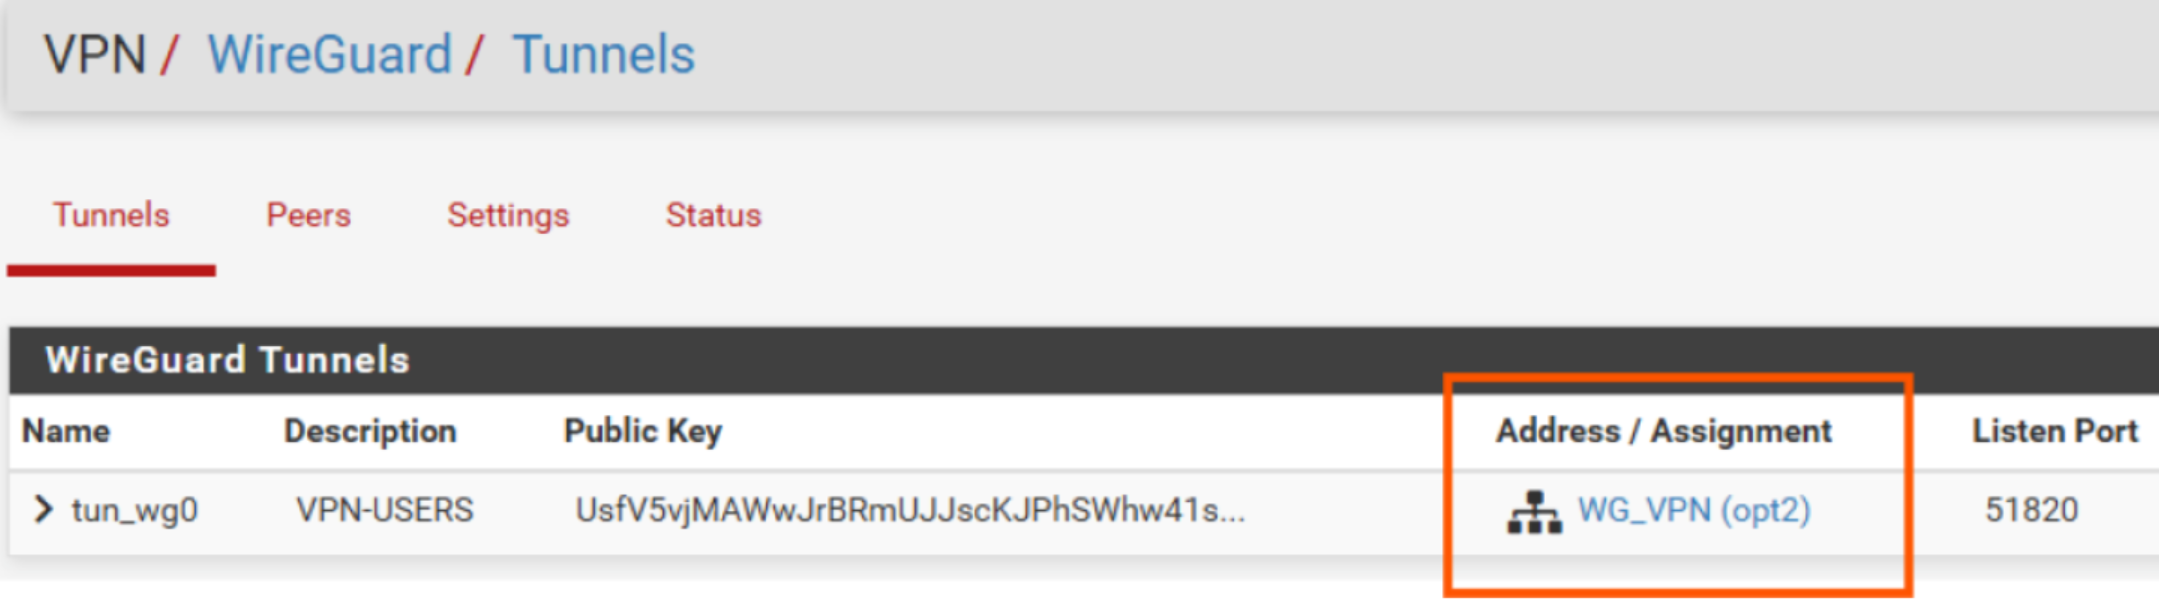
\includegraphics[width=0.8\textwidth]{contents/img/interface_wg_save.png}
\end{center}

\vspace{0.5cm}

\noindent Si vous regardez votre tunnel WireGuard vous verrez qu'il est maintenant associé à l'interface.

\vspace{0.5cm}

\noindent La MTU standard d’Ethernet est souvent 1500 octets.

\noindent Lorsqu’on utilise un tunnel VPN (par exemple IPsec, OpenVPN, WireGuard), il y a un en-tête supplémentaire ajouté aux paquets pour gérer le chiffrement et l’encapsulation.

\noindent Ces en-têtes VPN prennent de la place (parfois entre 40 et 80 octets ou plus).

\noindent Donc, pour que les paquets VPN ne soient pas fragmentés à l’intérieur du tunnel, on réduit la MTU à une valeur plus petite, par exemple autour de 1420 octets.

\vspace{0.5cm}

Questions~: Savez vous ce qu'est le MTU ? et pourquoi il est à 1420 ci-dessus ?

\vspace{0.5cm}

\noindent \textbf{Maximum Transmission Unit}

\noindent La valeur de MTU en réseau signifie Maximum Transmission Unit (Unité de Transmission Maximale).

\noindent C’est la taille maximale en octets qu’un paquet de données (ou trame) peut avoir pour être transmis sur un réseau sans être fragmenté

\noindent \textbf{MTU à 1420}

\noindent La MTU standard d’Ethernet est souvent 1500 octets.

\noindent Lorsqu’on utilise un tunnel VPN (par exemple IPsec, OpenVPN, WireGuard), il y a un en-tête supplémentaire ajouté aux paquets pour gérer le chiffrement et l’encapsulation.

\noindent Ces en-têtes VPN prennent de la place (parfois entre 40 et 80 octets ou plus).

\noindent Donc, pour que les paquets VPN ne soient pas fragmentés à l’intérieur du tunnel, on réduit la MTU à une valeur plus petite, par exemple autour de 1420 octets. Ceci améliore la performance et la stabilité.

\newpage

\subsection*{Activation de Wireguard}
\phantomsection
\addcontentsline{toc}{subsection}{Activation de Wireguard}

\noindent Le service Wireguard ne s'active pas par défaut. Vous devez utiliser \textbf{VPN > WireGuard > Settings} et cocher \textbf{Enable Wireguard} puis cliquer sur \textbf{Save}.

\vspace{0.5cm}

\begin{center}
  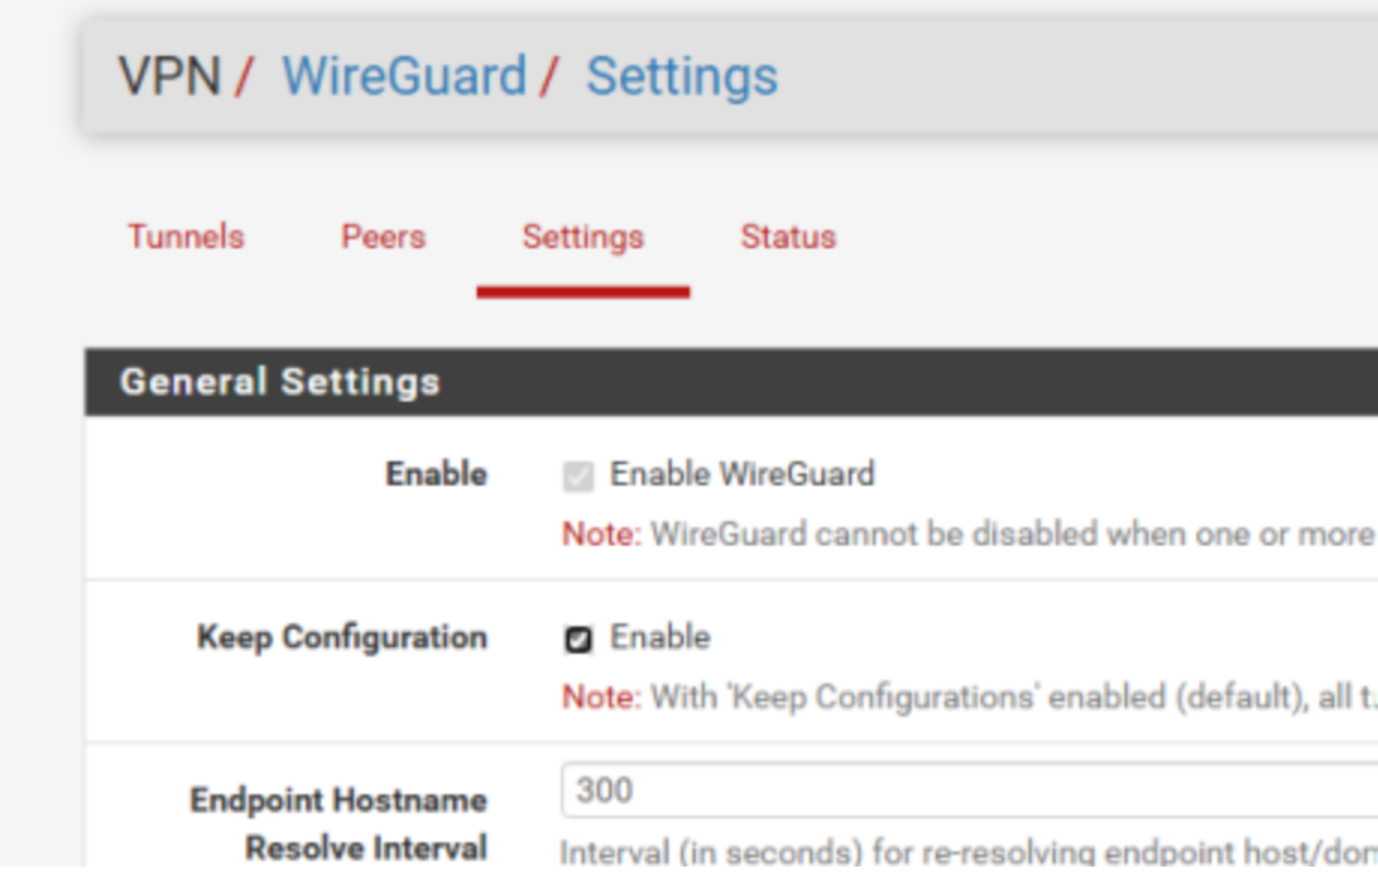
\includegraphics[width=0.8\textwidth]{contents/img/enable_wiregard.png}
\end{center}

\vspace{0.5cm}

\subsection*{Configuration des clients VPN WireGard sur les PC}
\phantomsection
\addcontentsline{toc}{subsection}{Configuration des clients VPN WireGard sur les PC}

\noindent Les utilisateurs en télétravail vont utiliser leur PC et leur connexion internet pour accéder au réseau local de leur entreprise. Il existe différentes façons de se connecter à un serveur VPN. Dans ce contexte, le client WireGuard va être installé et utilisé sur les PC des utilisateurs. La corbeille utilise votre PC et donc vous allez installer le client sur votre PC.

\noindent \textbf{Prérequis}

\noindent Pour configurer le client, vous devez connaître l'adresse IP WAN de l'interface de la VM pfSense en mode Bridged qui a obtenu une adresse IP en DHCP. Vous devez pouvoir la joindre à partir de votre PC fixe.

\noindent Sur l'interface d'administration de la VM pfSense, utilisez \textbf{Status>Interfaces} puis notez l'adresse IP de Wan Interface.

\vspace{0.5cm}

\begin{center}
  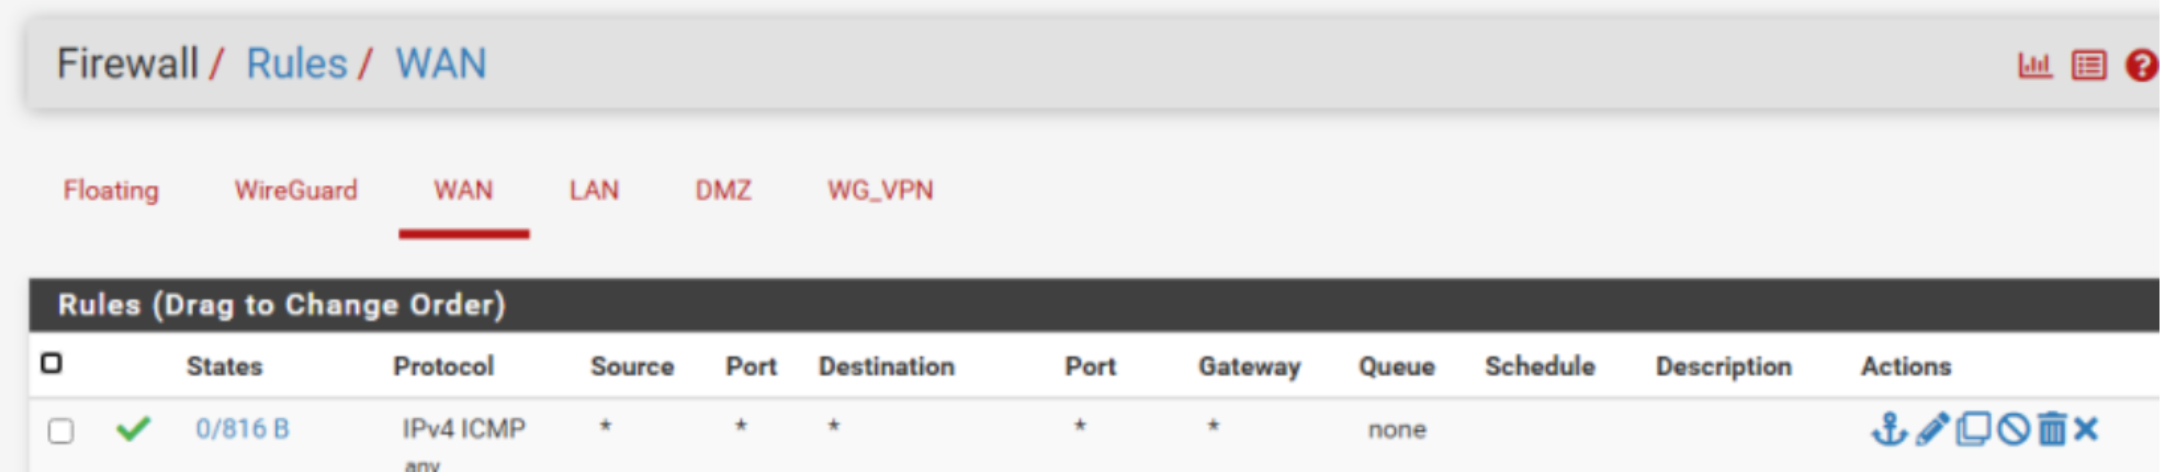
\includegraphics[width=0.6\textwidth]{contents/img/wan_ip_pfsense.png}
\end{center}

\noindent Dans le cadre de la corbeille à des fins de diagnostic vous pouvez autoriser ICMP sur l'interface WAN et tester si votre PC peut utiliser ping pour la joindre

\noindent Exemple : une interface WAN ayant ici une adresse IP 192.168.1.128 doit pouvoir être jointe de votre PC physique.

\vspace{0.5cm}

\begin{center}
  \begin{verbatim}
    ping 192.168.1.128

    Envoi d’une requête 'Ping' 192.168.1.128 avec 32 octets de données :
    Réponse de 192.168.1.128 : octets=32 temps<1ms TTL=64
    Réponse de 192.168.1.128 : octets=32 temps=1 ms TTL=64
    Réponse de 192.168.1.128 : octets=32 temps=3 ms TTL=64
    Réponse de 192.168.1.128 : octets=32 temps=2 ms TTL=64
  \end{verbatim}
\end{center}

\noindent Essayez de joindre la VM serveur sur le réseau LAN virtuel (192.198.74.0/24). Normalement vous ne devez pas y arriver.

\noindent Évidemment, en partant du principe que vous avez autorisé ICMP sur le pare-feu Windows.

\noindent Vous devez maintenant :
\begin{itemize}
  \item Télécharger et installer le client Wireguard sur votre PC
  \item Configurer les informations du tunnel sur le client installé (en utilisant la clé publique du Tunnel et l'adresse IP de l'interface WAN)
\end{itemize}

\vspace{0.5cm}

\begin{center}
  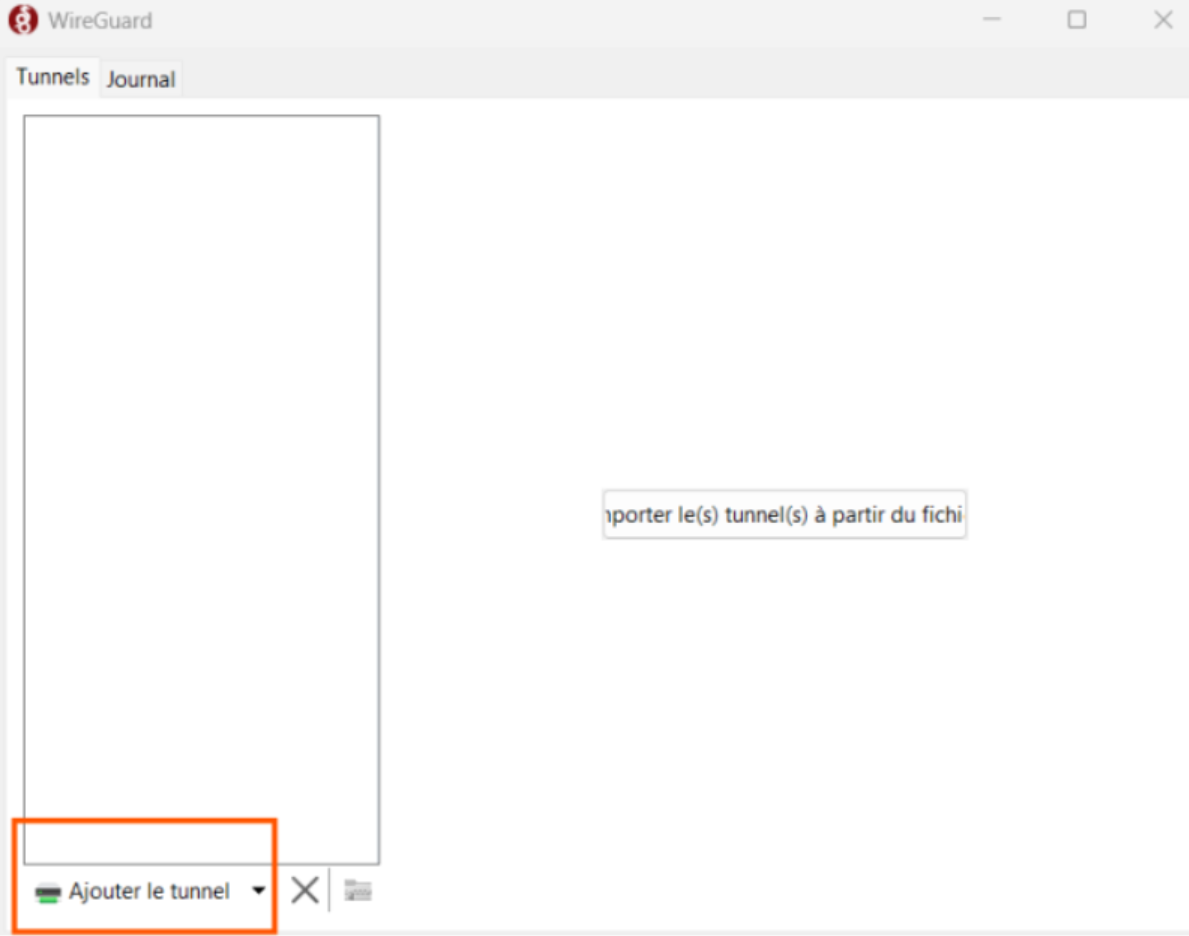
\includegraphics[width=0.6\textwidth]{contents/img/wireguard_client_config.png}
\end{center}

\begin{itemize}
  \item Lancez le client WireGard.
  \item Cliquez sur Ajouter un tunnel puis Ajouter un tunnel vide
\end{itemize}

\vspace{0.5cm}

\begin{center}
  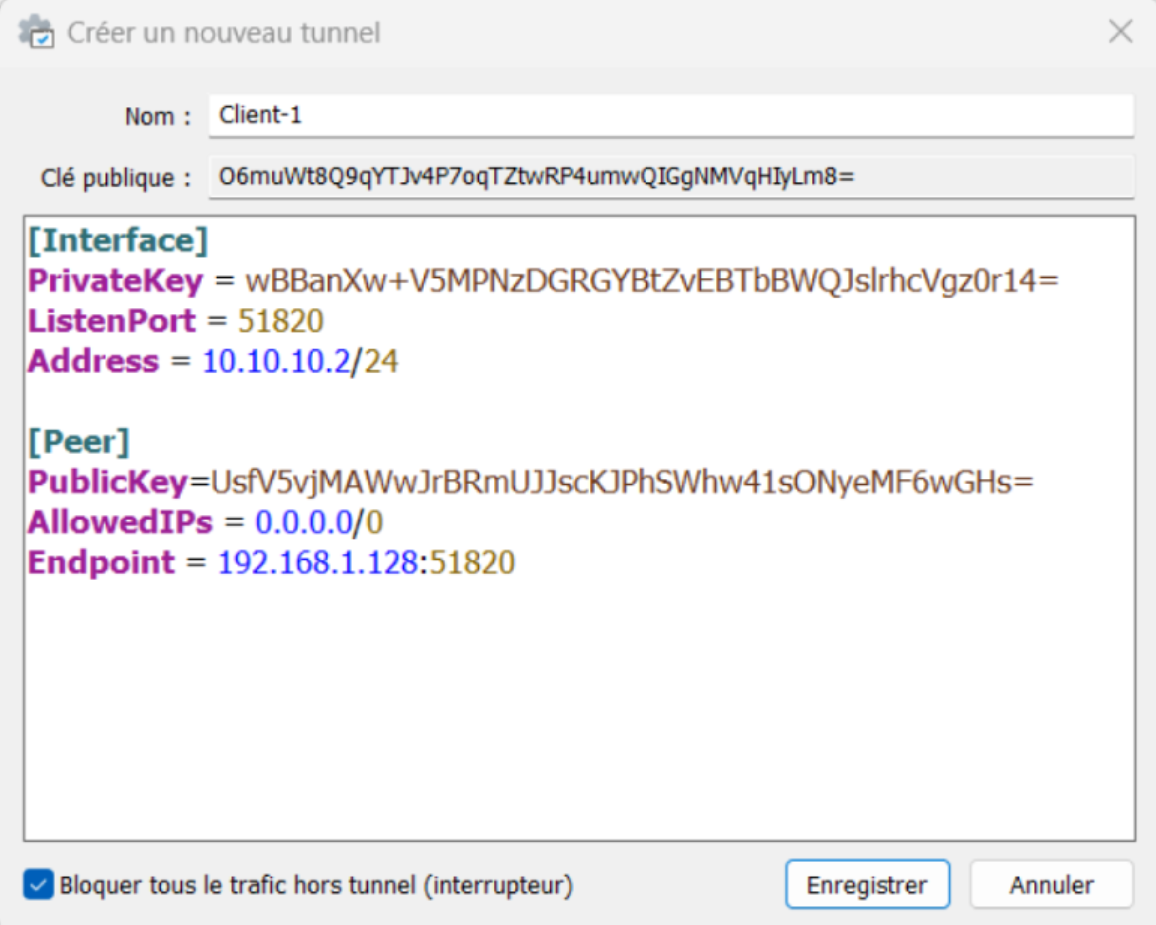
\includegraphics[width=0.6\textwidth]{contents/img/wireguard_client_config_2.png}
\end{center}

\begin{itemize}
  \item Donnez un nom à votre client, ici par exemple Client-1 
  \item Renseigner les informations de votre Tunnel VPN sur le Client : 
\end{itemize}

\vspace{0.5cm}

\noindent \textbf{Interface}
\begin{itemize}
  \item PrivateKey = Garder la Clé privée proposée
  \item ListenPort = 51820 (Port d’écoute du Tunnel VPN)
  \item Address = 10.10.10.1/24 (Adresse IP disponible du Tunnel VPN au format CIDR)
\end{itemize}

\noindent \textbf{Peer}
\begin{itemize}
  \item PublicKey = Coller la Clé Publique « Public Key » du Tunnel VPN définie dans le tunnel WireGard
  \item AllowedIPs = 0.0.0.0/0 (Autorise toutes les adresses IP)
  \item Endpoint = 192.168.1.1:51820
\end{itemize}

\noindent (Adresse IP WAN Publique du Serveur pfSense WireGuard suivie du Port d’écoute du Tunnel VPN).

\vspace{0.5cm}

\begin{center}
  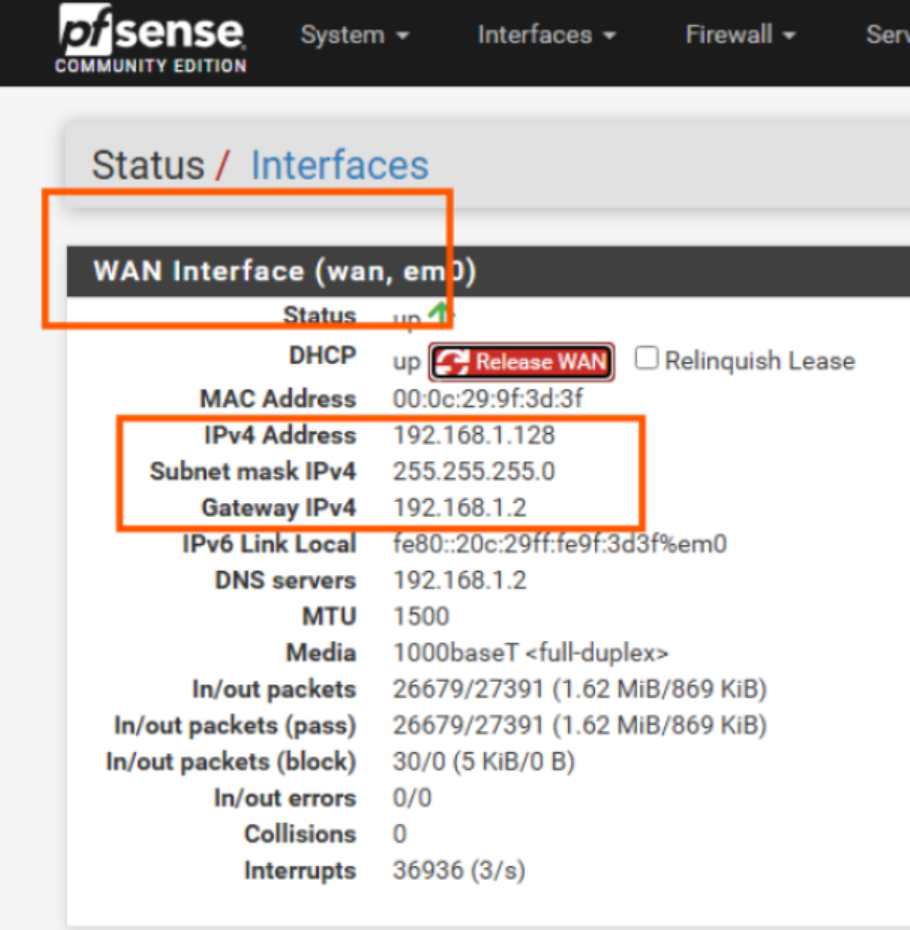
\includegraphics[width=0.6\textwidth]{contents/img/wireguard_client_config_save.png}
\end{center}

\noindent Cliquez sur Save pour enregistrer la configuration du client VPN.

\begin{center}
  \begin{verbatim}
    [Interface]
    PrivateKey = wBBanXw+V5MPNzDGRGYBtZvEBTbBWQJslrhcVgz0r14=
    ListenPort = 51820
    Address = 10.10.10.2/24

    [Peer]
    PublicKey=UsfV5vjMAWwJrBRmUJJscKJPhSWhw41sONyeMF6wGHs=
    AllowedIPs = 0.0.0.0/0
    Endpoint = 192.168.1.128:51820
  \end{verbatim}
\end{center}

\vspace{0.5cm}

\begin{center}
  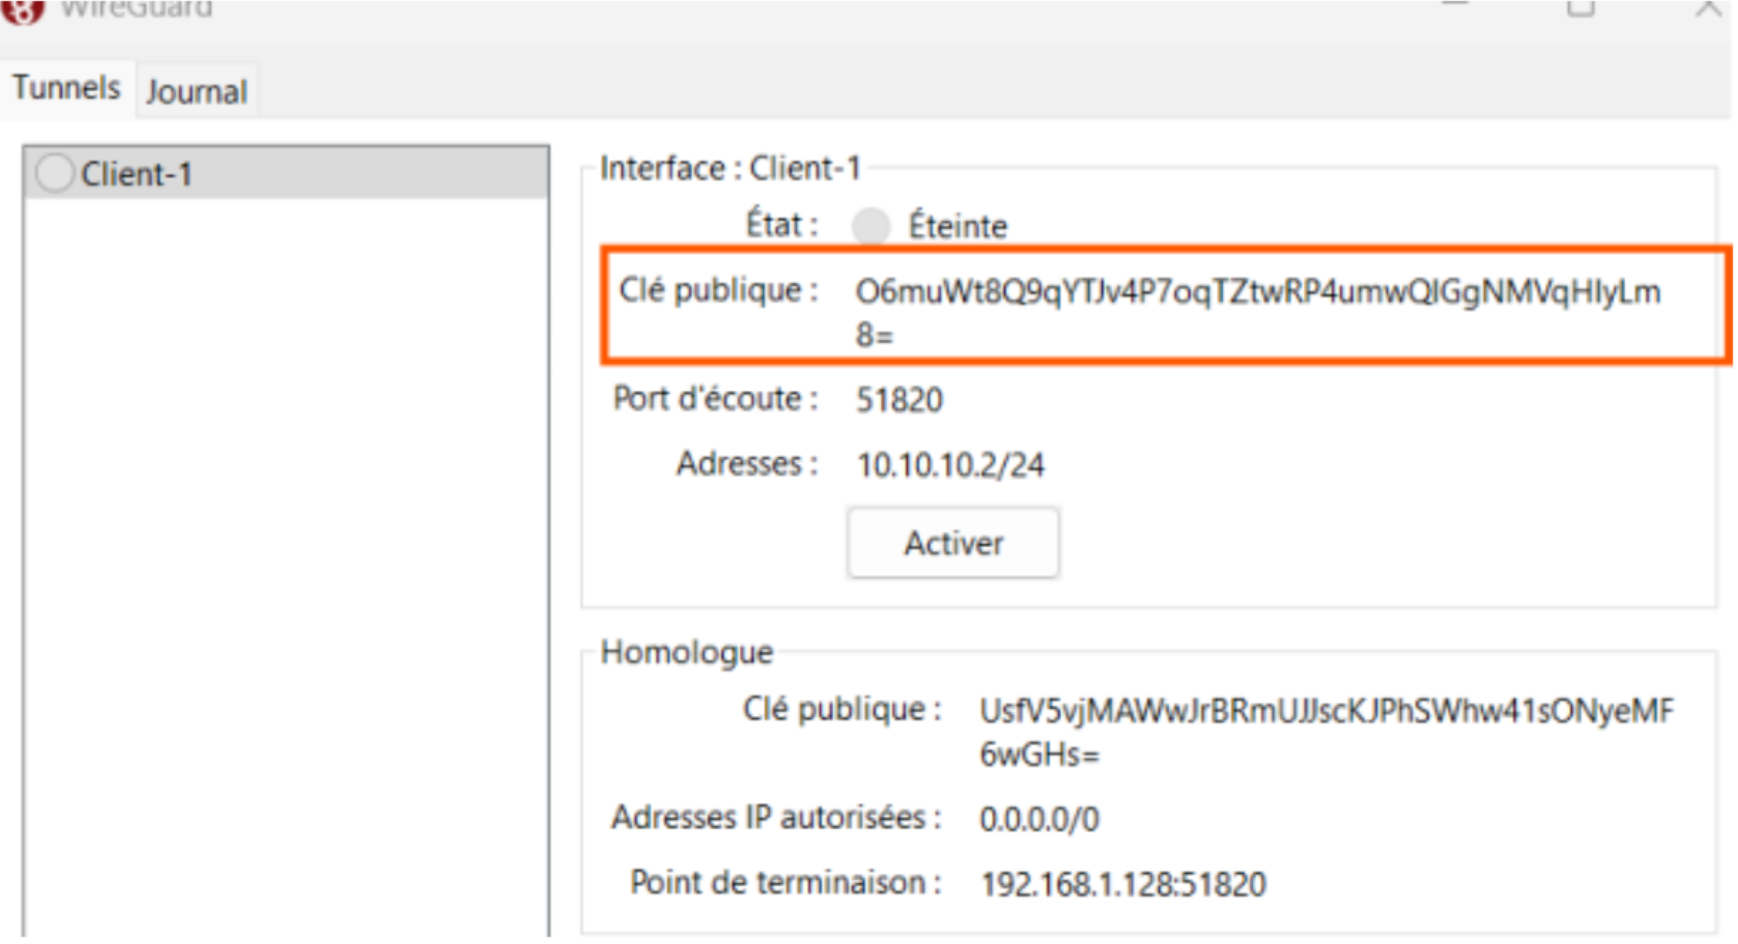
\includegraphics[width=0.6\textwidth]{contents/img/wireguard_client_activate.png}
\end{center}

\vspace{0.5cm}

\noindent Copiez la Clé publique du client.

\newpage

\noindent Vous devez maintenant configurer un peer. Dans un VPN (comme WireGuard) un peer est un participant au tunnel VPN :

\begin{itemize}
  \item Soit un client (c'est votre cas)
  \item Soit un serveur
  \item Ou même un autre routeur dans un VPN site-à-site
\end{itemize}

\noindent Chaque peer est défini par :
\begin{itemize}
  \item Une clé publique,
  \item Une adresse IP dans le tunnel VPN,
  \item Une adresse IP publique à contacter (ici l'adresse WAN),
  \item Des règles de routage (quels réseaux il peut atteindre via ce peer).
\end{itemize}

\vspace{0.5cm}

\noindent \textbf{Donc vous allez créer un pair sur le serveur VPN pfSense associé à l'adresse IP et la clé publique de votre client VPN.}

\vspace{0.5cm}

\begin{center}
  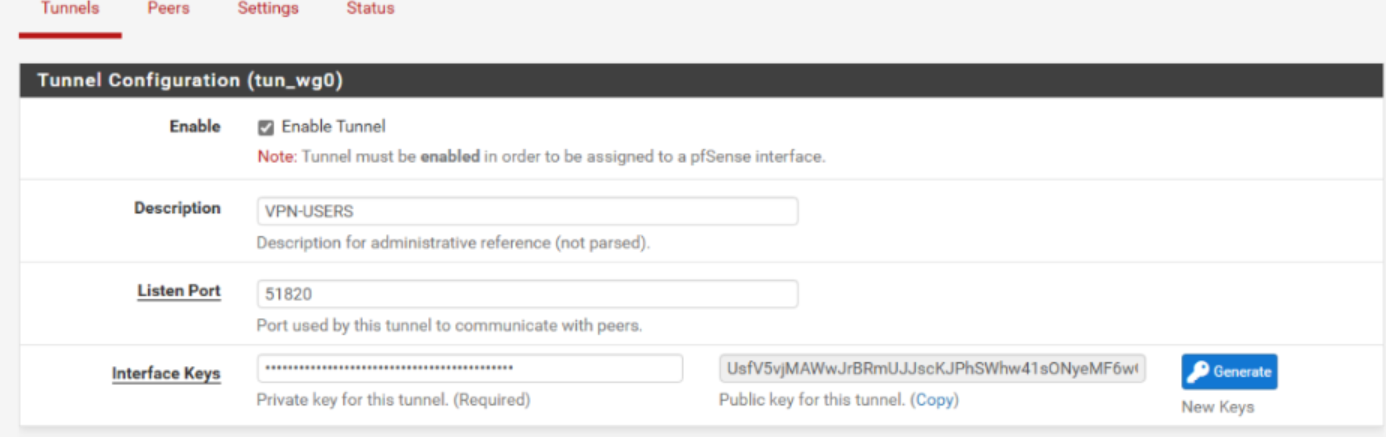
\includegraphics[width=0.8\textwidth]{contents/img/wireguard_add_peer.png}
\end{center}

\vspace{0.5cm}

\begin{itemize}
  \item Sur l'interface web du serveur pfSense. Choisissez \textbf{VPN/WireGard/Tunnel}
  \item Editez le tunnel dans \textbf{Action}.
  \item Dans Peer Configuration en bas de l'écran, cliquez sur \textbf{+Add Peer}
\end{itemize}

\vspace{0.5cm}

\begin{center}
  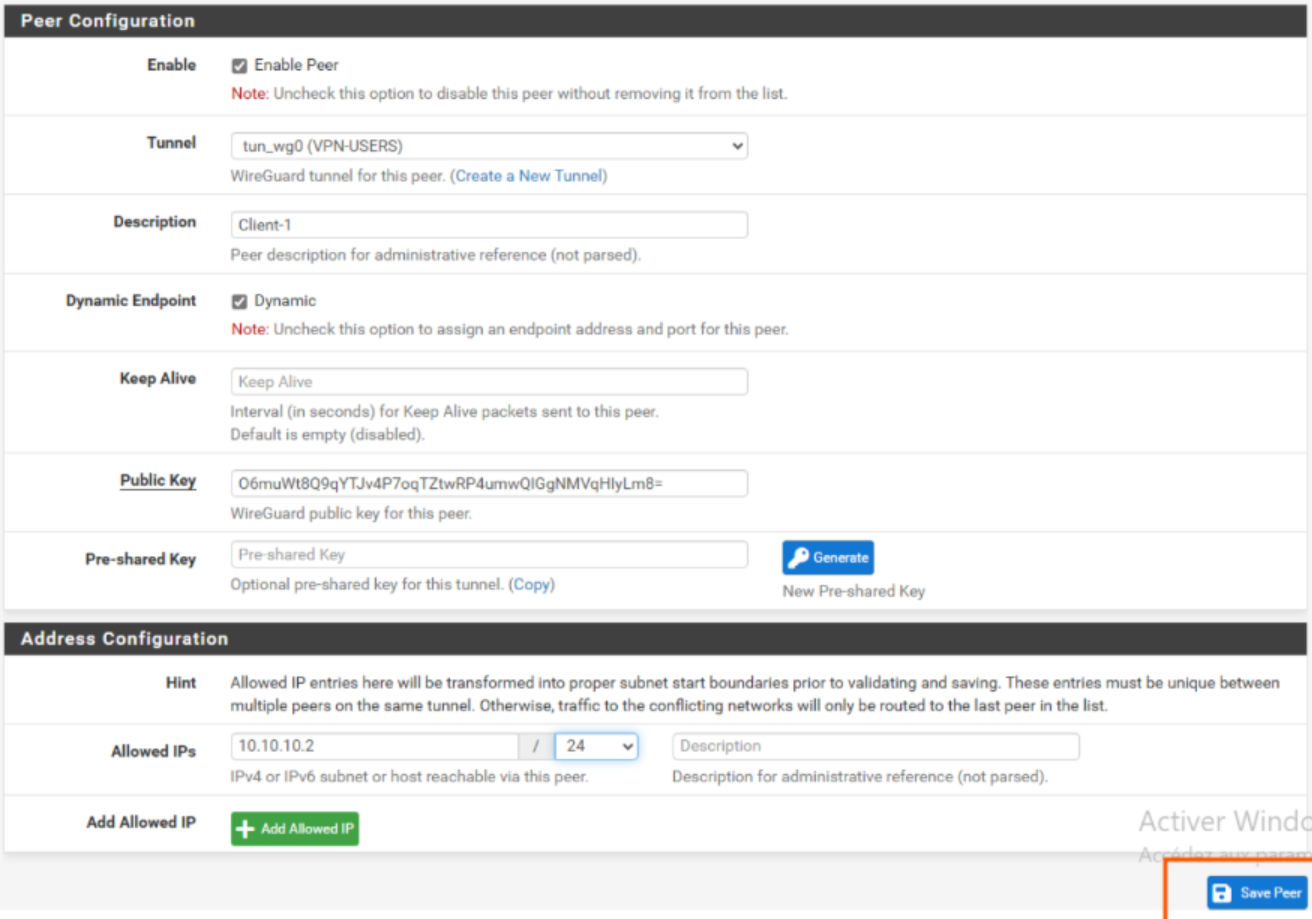
\includegraphics[width=0.6\textwidth]{contents/img/wireguard_add_peer_config.png}
\end{center}

\vspace{0.5cm}

\begin{itemize}
  \item Entrez une Description (Client-1)
  \item Endpoint : Laissez vide pour les points de terminaison dynamiques
  \item Keep Alive : Laissez vide. (Utile pour vérifier que le Tunnel VPN est toujours actif)
  \item Public Key : Collez la « Clé Publique » du Client
  \item Allowed IPs : 10.10.10.2/32 (Adresse IP du Client au format CIDR)
  \item Cliquer sur Update
\end{itemize}

\subsection*{Configurer les règles du pare-feu pfSense}
\phantomsection
\addcontentsline{toc}{subsection}{Configurer les règles du pare-feu pfSense}

\noindent L'objectif du client VPN est de permettre un accès au poste distant aux ressources du LAN. Il est nécessaire de mettre en place plusieurs règles de filtrage à paramétrer via l'interface d'administration de la VM pfSense.

\begin{itemize}
  \item Création d’une règle pour autoriser les clients à monter la connexion VPN
  \item Création d’une règle pour autoriser l’accès aux ressources coté WAN.
\end{itemize}

\vspace{0.5cm}

Question~: Quelle est la règle à mettre en place sur l'interface WAN pour autoriser la connexion VPN ? (autoriser le trafic pour accéder au service WireGuard). Vous avez normalement toutes les informations nécessaires, le port et le protocole.

\noindent Pouvez vous la mettre en place ?

\vspace{0.5cm}

\noindent \textbf{UDP 51820}

\noindent Il faut ajouter une règle autorisant à un client VPN d'accéder au serveur VPN sur l'interface WAN du pfSense.

\noindent Il faut donc autoriser le trafic UDP sur le port utilisé par WireGuard (51820 par défaut).

\noindent \textbf{Création de la règle}

\noindent Utilisez le menu \textbf{Firewall > Rules > WAN} (l’interface qui reçoit le trafic VPN).

\noindent Ajoutez une règle autorisant le trafic UDP sur le port utilisé par WireGuard (51820 par défaut).

\begin{itemize}
  \item Action : Pass
  \item Interface : WAN
  \item Protocol : \textbf{UDP}
  \item Source : any
  \item Destination : WAN address
  \item Destination Port Range – Custom : \textbf{51820}
  \item Cliquer sur \textbf{Save} et valider \textbf{Apply Changes}
\end{itemize}

\vspace{0.5cm}

Question~: Quelle(s) autre(s) règle(s) doive(nt) être mise(s) en place ? Quelles sont les interfaces dans le menu \textbf{Firewall>Rules} ?

\vspace{0.5cm}

\noindent \textbf{Interface WireGuard sur pfSense}

\noindent L’interface WireGuard sur pfSense représente une interface réseau virtuelle, qui permet de gérer les flux de données chiffrés passant par un tunnel VPN WireGuard.

\noindent \textbf{Firewall/Rules/WireGuard}

\noindent ne interface WireGuard est présente et a été créer automatiquement.

\noindent Vous devez créer les règles nécessaires à l'accès des clients VPN au LAN.

\begin{itemize}
  \item Action : Pass
  \item Interface : WireGuard
  \item Protocol : Any
  \item Source : any
  \item Destination : any
  \item Cliquer sur Save et valider Apply Changes
\end{itemize}

\newpage

\section*{Analyse et résolution : Chiffrement}
\addcontentsline{toc}{section}{Analyse et résolution : Chiffrement}

\subsection*{Analyser les besoins de sécurité pour GLPI}
\phantomsection
\addcontentsline{toc}{subsection}{Analyser les besoins de sécurité pour GLPI}

\noindent GLPI manipule des données internes sensibles telles que les tickets d'assistance, les inventaires et les comptes utilisateurs. Sa mise en production exige donc un niveau de sécurité strict. Les besoins principaux sont les suivants.

\begin{itemize}
  \item \textbf{Confidentialité}. Toutes les communications doivent impérativement être chiffrées via HTTPS, afin de protéger les identifiants et les données échangées entre les utilisateurs et le serveur.
  \item \textbf{Authentification centralisée}. L'utilisation de la base locale de GLPI n'est pas adaptée à un environnement d'entreprise. L'authentification via Active Directory, en LDAPS, permet un contrôle centralisé, la révocation rapide des comptes et une cohérence des droits.
  \item \textbf{Intégrité du système}. L'accès à l'interface doit être strictement contrôlé. Le chiffrement ne suffit pas: une segmentation réseau et un contrôle d'accès doivent empêcher toute modification non autorisée.
  \item \textbf{Disponibilité}. GLPI est un service critique pour le support. L'accès doit rester stable, y compris pour les utilisateurs distants, ce qui impose une architecture fiable et surveillée.
  \item \textbf{Traçabilité}. L'intégration à l'AD permet une journalisation complète des accès et des actions, conforme aux exigences internes.
\end{itemize}

\medskip

\subsection*{Étudier le fonctionnement théorique du chiffrement}
\phantomsection
\addcontentsline{toc}{subsection}{Étudier le fonctionnement théorique du chiffrement}

\noindent Le chiffrement des communications repose principalement sur TLS. Son fonctionnement suit une logique en deux temps.

\begin{itemize}
  \item \textbf{Établissement de la session}. Le client vérifie le certificat du serveur, le serveur prouve son identité via sa clé privée, puis une clé de session symétrique est négociée.
  \item \textbf{Chiffrement des données}. Une fois la clé de session établie, tout le trafic est chiffré avec des algorithmes symétriques (Ex. AES), garantissant la confidentialité et l'intégrité des données échangées.
\end{itemize}

\noindent Il ne faut pas confondre TLS avec SSH: ce sont deux protocoles distincts, utilisés pour des usages différents. HTTPS repose sur TLS, pas sur SSH.

\medskip

\subsection*{Étudier le fonctionnement théorique des certificats numériques}
\phantomsection
\addcontentsline{toc}{subsection}{Étudier le fonctionnement théorique des certificats numériques}

\noindent Un certificat X.509 contient l'identité du serveur, sa clé publique, une période de validité et la signature d'une autorité de certification (CA). Il ne chiffre pas les données: il sert à \textbf{authentifier} le serveur et à permettre un échange de clé sécurisé.

\begin{itemize}
  \item \textbf{Certificat auto-signé}. Le serveur se signe lui-même. Un navigateur ne fera jamais confiance à ce certificat, d'où l'avertissement observé sur GLPI.
  \item \textbf{Certificat interne}. Signé par la CA de l'entreprise, déjà approuvée sur les postes clients. Il supprime immédiatement les alertes de sécurité et reste adapté à un service interne.
  \item \textbf{Certificat public}. Signé par une CA mondialement reconnue. Nécessaire pour un service exposé sur Internet. Un certificat wildcard peut être utilisé pour couvrir plusieurs sous-domaines (\texttt{*.berria.org}).
\end{itemize}

\medskip

\subsection*{Comparer les solutions d'accès distant (VPN vs Publication Web sécurisée)}
\phantomsection
\addcontentsline{toc}{subsection}{Comparer les solutions d'accès distant (VPN vs Publication Web sécurisée)}

\noindent Deux approches principales permettent l'accès distant : une publication Web sécurisée ou l'utilisation d'un VPN.

\begin{itemize}
  \item \textbf{Publication Web sécurisée}. L'accès se fait via HTTPS ouvert sur Internet. L'avantage principal est la simplicité d'utilisation. Cependant, la surface d'expo-sition est plus large et nécessite un durcissement rigoureux du serveur (reverse-proxy, filtrage, mises à jour fréquentes) ainsi qu'un certificat public fiable.
  \item \textbf{VPN OpenVPN}. Les utilisateurs se connectent au réseau interne via un client VPN. Le serveur GLPI reste isolé dans le LAN des serveurs, et seule l'interface VPN expose un service au public. La sécurité est nettement supérieure, la surface d'attaque réduite et l'architecture mieux maîtrisée. Cette solution est également moins coûteuse à sécuriser. Pour BERRIA, elle est objectivement plus adaptée.
\end{itemize}

\newpage

\subsection*{Maquetter l'authentification LDAPS avec l'Active Directory}
\phantomsection
\addcontentsline{toc}{subsection}{Maquetter l'authentification LDAPS avec l'Active Directory}

\noindent La mise en place de l'authentification via LDAPS nécessite plusieurs prérequis techniques.

\begin{itemize}
  \item Vérifier que le contrôleur de domaine dispose d'un certificat serveur valide et approuvé.
  \item Tester le fonctionnement de LDAPS via \\ \texttt{openssl s\_client -connect ad.berria.local:636}.
  \item Configurer GLPI avec les paramètres LDAP: serveur, DN de base, attribut de connexion, mode LDAPS.
  \item Tester l'import d'utilisateurs et la synchronisation automatique.
\end{itemize}

\noindent La confiance envers le certificat du contrôleur de domaine est indispensable pour garantir un canal LDAPS fiable.

\medskip

\subsection*{Mettre en place la solution de certificat choisie (résolution de l'avertissement navigateur)}
\phantomsection
\addcontentsline{toc}{subsection}{Mettre en place la solution de certificat choisie (résolution de l'avertissement navigateur)}

\noindent L'avertissement actuel provient du certificat auto-signé utilisé par GLPI. Trois options existent.

\begin{itemize}
  \item \textbf{Certificat interne}. Le plus logique si GLPI reste interne. La DSI génère un certificat signé par la CA interne; les navigateurs le reconnaissent immédiatement.
  \item \textbf{Certificat public wildcard}. Pertinent si le service est publié sur Internet. Il bénéficie d'une confiance universelle.
  \item \textbf{Let's Encrypt}. Gratuit, mais utilisable seulement si le serveur est accessible publiquement.
\end{itemize}

\noindent Pour le contexte actuel, un certificat interne suffit largement si l'accès se fait via VPN.

\newpage

\subsection*{Configurer l'accès distant}
\phantomsection
\addcontentsline{toc}{subsection}{Configurer l'accès distant}

\noindent Deux scénarios existent selon le choix retenu.

\begin{itemize}
  \item \textbf{Accès via VPN}. Déployer ou réutiliser une infrastructure OpenVPN, distribuer les profils utilisateurs, restreindre le routage au seul réseau GLPI et ouvrir uniquement le port HTTPS du serveur aux utilisateurs connectés.
  \item \textbf{Publication Web}. Placer GLPI derrière un reverse-proxy durci, appliquer les bonnes pratiques TLS (TLS~1.2 minimum, désactivation des suites faibles), utiliser un certificat public et filtrer strictement les flux en DMZ.
\end{itemize}

\medskip

\subsection*{Tester et valider la solution finale}
\phantomsection
\addcontentsline{toc}{subsection}{Tester et valider la solution finale}

La validation finale impose les tests suivants.

\begin{itemize}
  \item Vérification de l'authentification LDAPS (connexion, révocation, import).
  \item Contrôle du certificat via un navigateur et test TLS (SSL Labs).
  \item Tests d'accès distant selon la solution retenue (VPN ou publication).
  \item Analyse réseau: scan externe pour vérifier que seul HTTPS est exposé.
  \item Tests de performance et de stabilité du service GLPI.
  \item Revue finale avec la DSI: conformité, coûts et risques résiduels.
\end{itemize}

\newpage 
\section*{Conclusion}
\addcontentsline{toc}{section}{Conclusion}

\noindent En conclusion, la mise en place d'une solution de sécurité robuste pour GLPI est essentielle pour protéger les données sensibles et garantir un accès sécurisé aux utilisateurs. Les études menées sur les différentes technologies de tunnelisation, telles que WireGuard et OpenVPN, ont démontré que l'utilisation d'un VPN offre une sécurité supérieure en isolant le serveur GLPI dans le réseau local tout en permettant un accès distant contrôlé. 

\noindent De plus, l'intégration de l'authentification LDAPS avec Active Directory renforce la sécurité en centralisant la gestion des identités et en assurant une communication chiffrée. Les certificats numériques jouent également un rôle crucial dans l'authentification des serveurs et la protection des échanges de données.

\noindent Enfin, la comparaison entre les solutions d'accès distant souligne que, bien que la publication Web sécurisée soit plus simple à mettre en œuvre, elle expose le serveur à des risques accrus. En revanche, un accès via VPN, associé à des pratiques de sécurité rigoureuses, constitue la solution la plus adaptée pour garantir la confidentialité, l'intégrité et la disponibilité des services GLPI.

\newpage

\section*{Capitalisation}
\addcontentsline{toc}{section}{Capitalisation}

\begin{center}
\setlength{\tabcolsep}{10pt}
\begin{tabular}{|p{0.25\textwidth}|p{0.50\textwidth}|m{0.08\textwidth}|}
\hline
\textbf{AAV} & \textbf{Commentaire} & \textbf{Statut} \\ \hline

Comparer différentes technologies de tunnelisation &
IPsec, OpenVPN et WireGuard étudiés en détail ; comparaison des avantages, inconvénients et cas d'usage fournie avec exemples pratiques sur Cisco Packet Tracer et pfSense. &
{\color{green!60!black}Acquis} \\ \hline

Construire une PKI &
Infrastructure complète couvrant CA racine, certificats serveur, certificats clients, révocation et validation ; processus de génération et gestion des clés expliqués avec OpenSSL. &
{\color{green!60!black}Acquis} \\ \hline

Expliquer le fonctionnement des certificats numériques &
Certificats X.509, auto-signés, internes et publics documentés ; rôle dans TLS, authentification serveur et résolution des alertes navigateur expliqués. &
{\color{green!60!black}Acquis} \\ \hline

Expliquer les termes de base liés à la cryptographie &
Glossaire complet fourni : chiffrement symétrique/asymétrique, hachage, TLS, SSH, SSL, signatures numériques, PKI avec définitions et applications. &
{\color{green!60!black}Acquis} \\ \hline

Appliquer un système de codage simple &
Bcrypt pour mots de passe, AES-256 pour chiffrement symétrique, ChaCha20 dans WireGuard ; exemples de configurations et bonnes pratiques intégrés. &
{\color{green!60!black}Acquis} \\ \hline

Sélectionner différentes solutions pour assurer la confidentialité &
Analyse complète VPN vs HTTPS direct ; accès distant via OpenVPN ou WireGuard ; authentification LDAPS vers Active Directory ; choix justifiés par la sécurité et la scalabilité. &
{\color{green!60!black}Acquis} \\ \hline

\end{tabular}
\end{center}

\newpage

\section*{Ressources}
\addcontentsline{toc}{section}{Ressources}
\begin{itemize}
  \item Tutoriel de configuration d’un NAT-Overload sur Cisco Packet Tracer : \\
  \url{https://ciscotracer.wordpress.com/2014/02/03/configuration-du-nat-overload-network-address-translation/}
  \item IPsec : \\
  \url{https://www.cisco.com/c/fr_ca/support/docs/security-vpn/ipsec-negotiation-ike-protocols/217432-understand-ipsec-ikev1-protocol.html }
  \item AES : \\
  \url{https://www.ssi.gouv.fr/entreprise/bonnes-pratiques/chiffrement/algorithmes-de-chiffrement/}
  \item VPN Site à Site : \\
  \url{https://www.cisco.com/c/en/us/td/docs/security/vpn_client/anyconnect/anyconnect46/administration/guide/b_AnyConnect_Administrator_Guide_4-6/configure-vpn.html}
  \item Certificat Auto-signé : \\
  \url{https://www.it-connect.fr/creer-un-certificat-auto-signe-sur-windows-server-2016/}
  \item Bcrypt : \\
  \url{https://cheatsheetseries.owasp.org/cheatsheets/Password_Storage_Cheat_Sheet.html#bcrypt}
  \item PKI : \\
  \url{https://docs.microsoft.com/fr-fr/windows-server/identity/ad-ds/manage/understand-the-components-of-active-directory-certificate-services}
  \item Intaller un package WireGuard : \\
  \url{https://docs.netgate.com/pfsense/en/latest/packages/wireguard/index.html}
\end{itemize}